%%%%%%%%%%%%%%%%%%%%%%%%%%%%%%%%%%%%%%%%%%%%%%%
%%%     Declarations (skip to Begin Document, line 88, for parts you fill in)
%%%%%%%%%%%%%%%%%%%%%%%%%%%%%%%%%%%%%%%%%%%%%%%

\documentclass[10pt]{article}

\usepackage{geometry}  % Lots of layout options.  See http://en.wikibooks.org/wiki/LaTeX/Page_Layout
\geometry{letterpaper}  % ... or a4paper or a5paper or ... 
\usepackage{fullpage}  % somewhat standardized smaller margins (around an inch)
\usepackage{setspace}  % control line spacing in latex documents
\usepackage[parfill]{parskip}  % Activate to begin paragraphs with an empty line rather than an indent
\usepackage{amsmath,amssymb}  % latex math
\usepackage{empheq} % http://www.ctan.org/pkg/empheq
\usepackage{bm,upgreek}  % allows you to write bold greek letters (upper & lower case)

\usepackage{url}

% allows strikethroughs in math via \cancel{math text goes here}
\usepackage{cancel}

% for typsetting algorithm pseudocode see http://en.wikibooks.org/wiki/LaTeX/Algorithms_and_Pseudocode
\usepackage{algorithmic,algorithm}  

\usepackage{graphicx}  % inclusion of graphics; see: http://en.wikibooks.org/wiki/LaTeX/Importing_Graphics
% allow easy inclusion of .tif, .png graphics
\DeclareGraphicsRule{.tif}{png}{.png}{`convert #1 `dirname #1`/`basename #1 .tif`.png}

%\usepackage{subfigure}  % allows subfigures in figure
\usepackage{caption}
\usepackage{subcaption}

\usepackage{xspace}
\newcommand{\latex}{\LaTeX\xspace}

\usepackage{color}  % http://en.wikibooks.org/wiki/LaTeX/Colors

\long\def\ans#1{{\color{blue}{\em #1}}}
\long\def\ansnem#1{{\color{blue}#1}}
\long\def\boldred#1{{\color{red}{\bf #1}}}
\long\def\boldred#1{\textcolor{red}{\bf #1}}
\long\def\boldblue#1{\textcolor{blue}{\bf #1}}
\long\def\todo#1{\textcolor{red}{\bf TODO: #1}}

% Useful package for syntax highlighting of specific code (such as python) -- see below
\usepackage{listings}  % http://en.wikibooks.org/wiki/LaTeX/Packages/Listings
\usepackage{textcomp}

%%% The following lines set up using the listings package
\renewcommand{\lstlistlistingname}{Code Listings}
\renewcommand{\lstlistingname}{Code Listing}

%%% Specific for python listings
\definecolor{gray}{gray}{0.5}
\definecolor{green}{rgb}{0,0.5,0}

\lstnewenvironment{python}[1][]{
\lstset{
language=python,
basicstyle=\footnotesize,  % could also use this -- a little larger \ttfamily\small\setstretch{1},
stringstyle=\color{red},
showstringspaces=false,
alsoletter={1234567890},
otherkeywords={\ , \}, \{},
keywordstyle=\color{blue},
emph={access,and,break,class,continue,def,del,elif ,else,%
except,exec,finally,for,from,global,if,import,in,i s,%
lambda,not,or,pass,print,raise,return,try,while},
emphstyle=\color{black}\bfseries,
emph={[2]True, False, None, self},
emphstyle=[2]\color{green},
emph={[3]from, import, as},
emphstyle=[3]\color{blue},
upquote=true,
morecomment=[s]{"""}{"""},
commentstyle=\color{gray}\slshape,
emph={[4]1, 2, 3, 4, 5, 6, 7, 8, 9, 0},
emphstyle=[4]\color{blue},
literate=*{:}{{\textcolor{blue}:}}{1}%
{=}{{\textcolor{blue}=}}{1}%
{-}{{\textcolor{blue}-}}{1}%
{+}{{\textcolor{blue}+}}{1}%
{*}{{\textcolor{blue}*}}{1}%
{!}{{\textcolor{blue}!}}{1}%
{(}{{\textcolor{blue}(}}{1}%
{)}{{\textcolor{blue})}}{1}%
{[}{{\textcolor{blue}[}}{1}%
{]}{{\textcolor{blue}]}}{1}%
{<}{{\textcolor{blue}<}}{1}%
{>}{{\textcolor{blue}>}}{1},%
%framexleftmargin=1mm, framextopmargin=1mm, frame=shadowbox, rulesepcolor=\color{blue},#1
framexleftmargin=1mm, framextopmargin=1mm, frame=single,#1
}}{}
%%% End python code listing definitions

\DeclareMathOperator{\diag}{diag}
\DeclareMathOperator{\cov}{cov}

%%%%%%%%%%%%%%%%%%%%%%%%%%%%%%%%%%%%%%%%%%%%%%%
%%%     Begin Document
%%%%%%%%%%%%%%%%%%%%%%%%%%%%%%%%%%%%%%%%%%%%%%%

\begin{document}

\vspace{1cm}

\begin{center}
    {\Large {\bf Loan Prediction System for Banks}} \\ 
\end{center}
\title{Loan Prediction System for Banks}


\section*{Abstract}

This project delves into the development and implementation of a Loan Prediction System for banks, leveraging the power of machine learning to enhance the efficiency and accuracy of loan approval processes. The primary objective is to address the pivotal questions faced by lending institutions: evaluating the risk associated with borrowers and determining the appropriateness of extending loans to them. By constructing predictive models, this project aims to streamline decision-making, optimize resource utilization, and mitigate the financial risks inherent in the loan approval process.

\section*{Introduction}

The proposal method aims to develop a robust and accurate loan prediction system for banks utilizing machine learning algorithms. The system's core functionality involves the analysis of historical customer data, including credit history, income, loan amount, loan term, and employment status, to predict the likelihood of a loan applicant receiving approval. The primary objective is to assist banks in making informed and reliable lending decisions, thereby reducing the risk of financial losses and streamlining the loan approval process.

The successful implementation of the loan prediction system holds the potential to empower banks to make data-driven decisions, minimize risks associated with loan defaults, optimize lending processes, and ultimately enhance their overall financial performance.

In addressing the specific problem presented by Comfort Zone company, the project seeks to automate the loan eligibility process in real-time based on customer details provided during online application submissions. By identifying eligible customer segments, the company aims to target specific customers efficiently. The overarching goal of the project is to predict whether a loan application would be approved or denied.

The lending industry faces two critical questions: How risky is the borrower, and given the borrower's risk, should the loan be granted? In response to these challenges, the project leverages data science teams in banks to build predictive models using machine learning techniques. Loan Prediction, a common real-life problem for retail banks, has the potential to save significant man-hours when approached correctly.

The proposed methodology and analysis plan include key components such as data collection, preprocessing, feature selection, model training, model evaluation, and continuous improvement. These steps are designed to gather historical loan applicant data, clean and prepare the data for analysis, identify relevant features impacting loan approval, train machine learning models, evaluate model performance, and implement mechanisms for continuous improvement.

In conclusion, the implementation of this system holds the promise of reducing the risk of financial losses associated with loan defaults, optimizing the loan approval process, and enhancing the overall operational effectiveness of banks. Through continuous improvement and adaptation to evolving market dynamics, the system aims to ensure its relevance over time.

\section*{Models}

The loan prediction system proposed in this project employs several machine learning models to address the specific challenges posed by the lending industry. The models selected for this project are tailored to handle classification problems, specifically binary classification, as the primary goal is to predict whether a loan application will be approved or denied.

\subsection*{Logistic Regression}

Logistic Regression is a fundamental classification algorithm that is well-suited for binary outcomes. In the context of this project, it will be utilized to model the probability of loan approval based on various independent variables such as credit history, income, and loan amount.

\[
P(Y=1) = \frac{1}{1 + e^{-(\beta_0 + \beta_1X_1 + \beta_2X_2 + \ldots + \beta_nX_n)}}
\]

\subsection*{Decision Trees}

Decision Trees are powerful tools for classification tasks, providing a clear and interpretable decision-making structure. In this project, Decision Trees will be employed to analyze and classify loan applications based on features like credit history, income, and other relevant factors.
\[
Decision \hspace{0.2cm} at \hspace{0.2cm} node \hspace{0.2cm} j: \quad X_i \leq t_j \, ?\]


\subsection*{K-Means Clustering}

While traditionally used for clustering, K-Means can also be adapted for classification tasks. In this project, K-Means Clustering will be explored to group similar loan applications and identify patterns that may influence the approval or denial of loans.
\[
J = \sum_{i=1}^{k} \sum_{j=1}^{n_i} ||x_{ij} - c_i||^2
\]


\subsection*{Model Selection Rationale}

The choice of these models is motivated by the need for interpretable results, the ability to handle diverse types of data, and the potential for achieving high predictive accuracy. Logistic Regression provides transparency in understanding the impact of each variable, while Decision Trees offer a visual representation of decision-making. K-Means Clustering, although primarily a clustering algorithm, will be explored for its potential in grouping similar loan applications.

These models collectively contribute to the overarching objective of predicting loan approval outcomes with precision, recall, and accuracy, ultimately assisting lending institutions in making well-informed decisions while minimizing the risk of financial losses.

\section*{Data}

The dataset used in this project consists of two CSV files: \texttt{train} and \texttt{test}. These files play a crucial role in training the machine learning models and evaluating their performance. The \texttt{train} file is employed for training the models, containing both the independent variables and the target variable. On the other hand, the \texttt{test} file includes only the independent variables, and the model's task is to predict the target variable for this test data.

Dataset Link: \url{https://www.kaggle.com/datasets/altruistdelhite04/loan-prediction-problem-dataset/data}

\subsection*{Dataset Variables}

The dataset comprises the following variables, each with its associated data type:
\begin{table}[h]
    \centering
    \begin{tabular}{|l|l|p{6cm}|}
        \hline
        \textbf{Variable} & \textbf{Data Type} & \textbf{Description} \\
        \hline
        Loan\_ID & Object & Unique Loan ID \\
        Gender & Object & Gender of the applicant \\
        Married & Object & Applicant's marital status \\
        Dependents & Object & Number of dependents \\
        Education & Object & Applicant's education level \\
        Self\_Employed & Object & Indicates whether the applicant is self-employed \\
        ApplicantIncome & Int & Income of the applicant \\
        CoapplicantIncome & Float & Income of the coapplicant \\
        LoanAmount & Float & Required loan amount in thousands \\
        Loan\_Amount\_Term & Float & Term of the loan in months \\
        Credit\_History & Float & Credit history of the applicant \\
        Property\_Area & Object & Urban/Semi Urban/Rural property area \\
        Loan\_Status & Object & Loan approval status (Target Variable) \\
        \hline
    \end{tabular}
    \caption{Data description of the variables in the dataset}
    \label{tab:description}
\end{table}


\subsection*{Data Structure}

The data is structured in rows and columns, with each row representing an individual loan application, and each column representing a specific attribute or feature. The \texttt{Loan\_Status} variable in the \texttt{train} file serves as the target variable that the machine learning models aim to predict.

The machine learning models will be trained on historical data from the \texttt{train} file, learning patterns and relationships between various features and the loan approval outcome. Subsequently, these models will be applied to the \texttt{test} file to predict the loan approval status for new, unseen data.

Understanding the nuances of each variable and the relationships within the dataset is essential for the successful development and deployment of the loan prediction system.

\section*{Procedure}

The implementation of the loan prediction system involves a systematic procedure. The primary machine learning models employed in this project include Logistic Regression, Decision Trees, and K-Means Clustering. Each model serves a specific purpose in predicting loan approval outcomes based on historical customer data.

\subsection*{Implementation Steps}

The implementation procedure follows key steps:

\begin{enumerate}
    \item \textbf{Data Collection:} Using historical loan applicant data, including both approved and denied loan applications, from the bank's existing database.\\
    Includes Univariate and Bivariate analysis of the Individual attributes of the dataset as shown through the below plots:

    \subsection*{Univariate Analysis}
\begin{figure}[H]
\begin{center}
        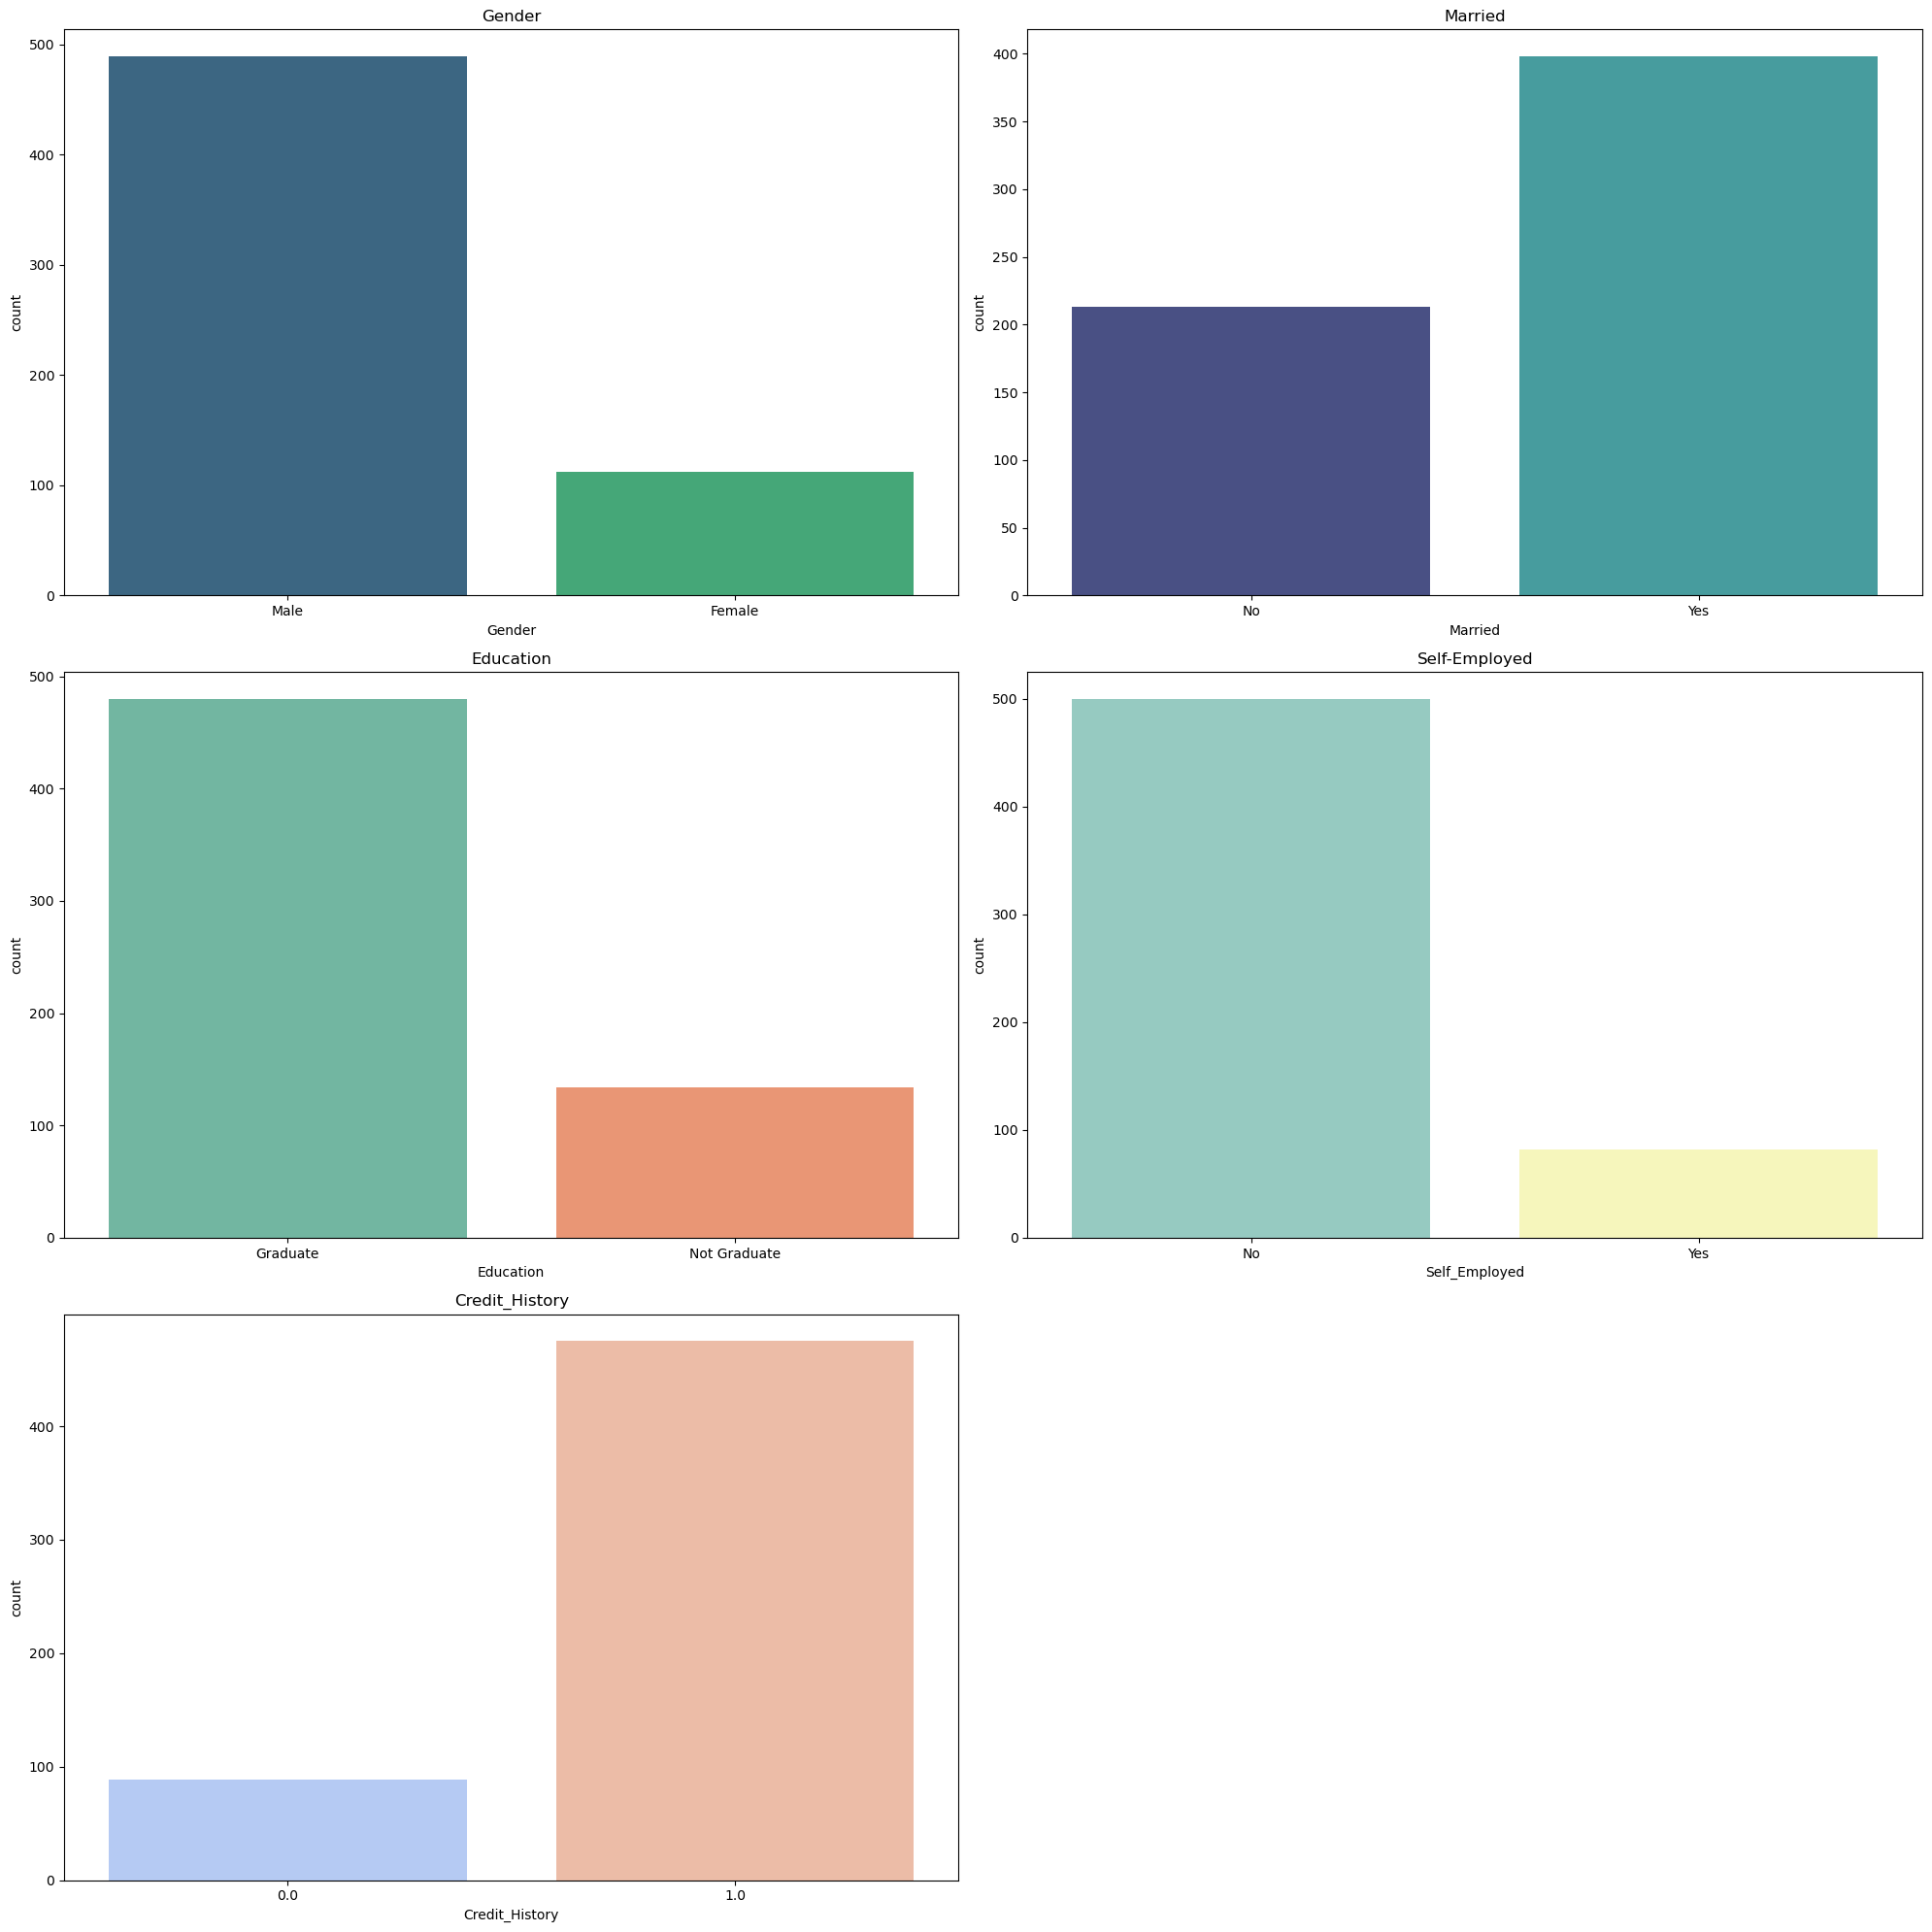
\includegraphics[width=15cm]{Columns_in_dataframe.png}
        \caption{Data Frame plotting different attributes}
        \label{fig:sub1}
\end{center}
\end{figure}
\begin{figure}[H]
\begin{center}
        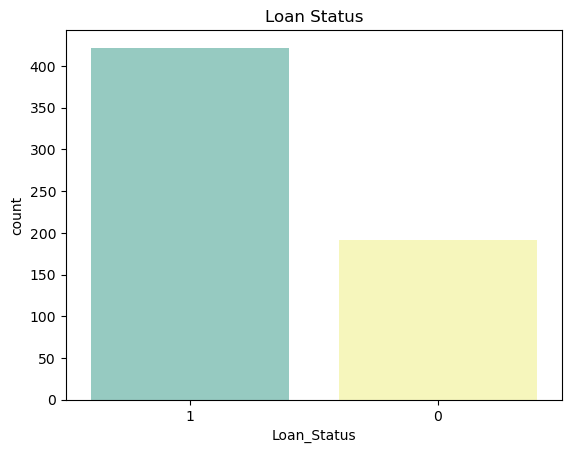
\includegraphics[width=0.4\linewidth]{Loan_Status_count.png}
        \caption{Target Value: Loan Status}
        \label{fig:sub1}
\end{center}
\end{figure}
\begin{figure}[H]
\begin{center}
        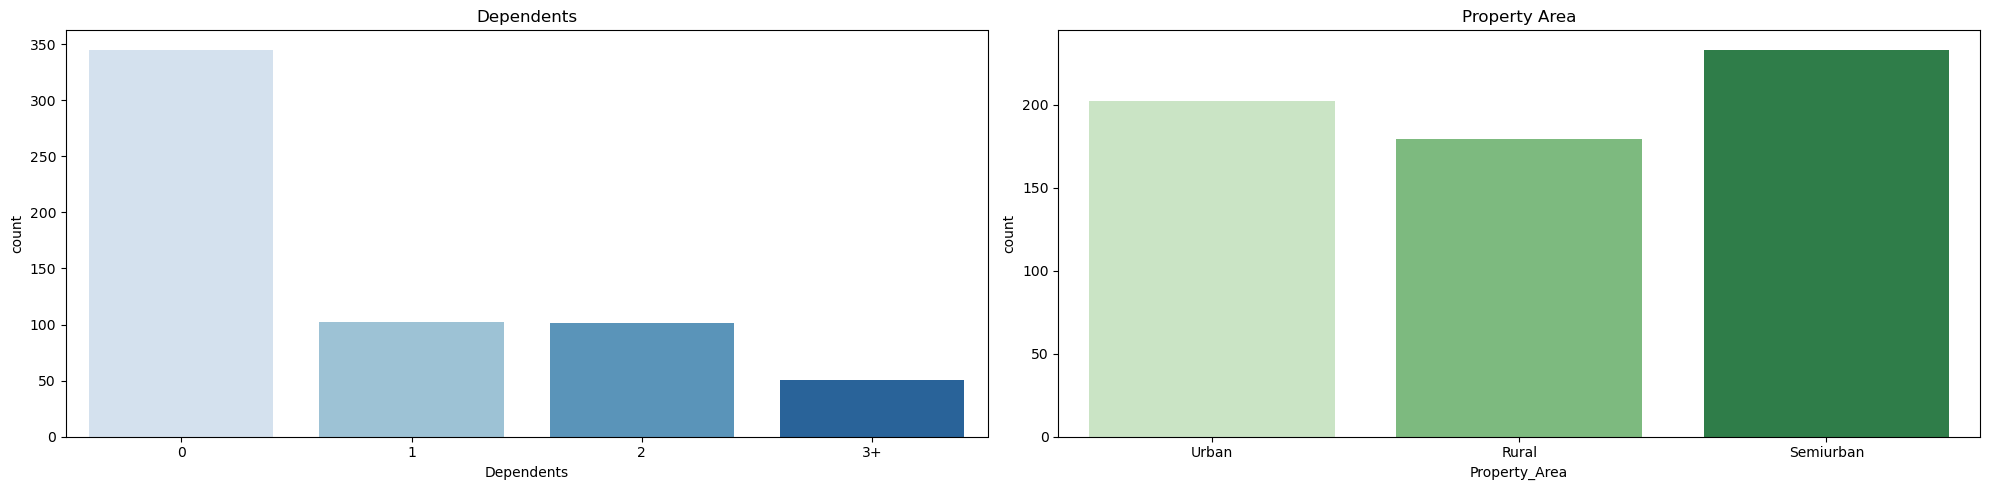
\includegraphics[width=15cm]{dependents_PropertyArea.png}
        \caption{Target Value: Dependents and Property Area Plot}
        \label{fig:sub1}
\end{center}
\end{figure}
\begin{figure}[H]
\begin{center}
        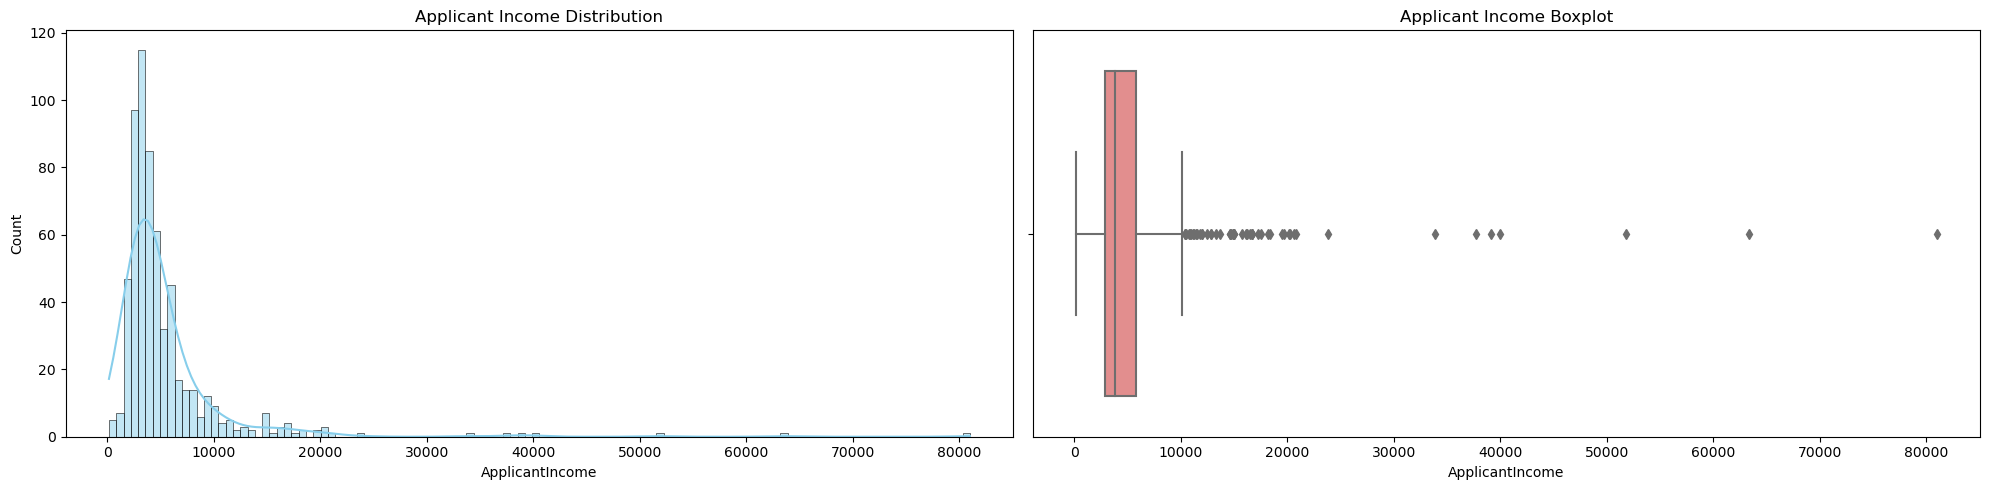
\includegraphics[width=15cm]{Applicant_Income.png}
        \caption{Target Value: Applicant Income}
        \label{fig:sub1}
\end{center}
\end{figure}
\begin{figure}[H]
\begin{center}
        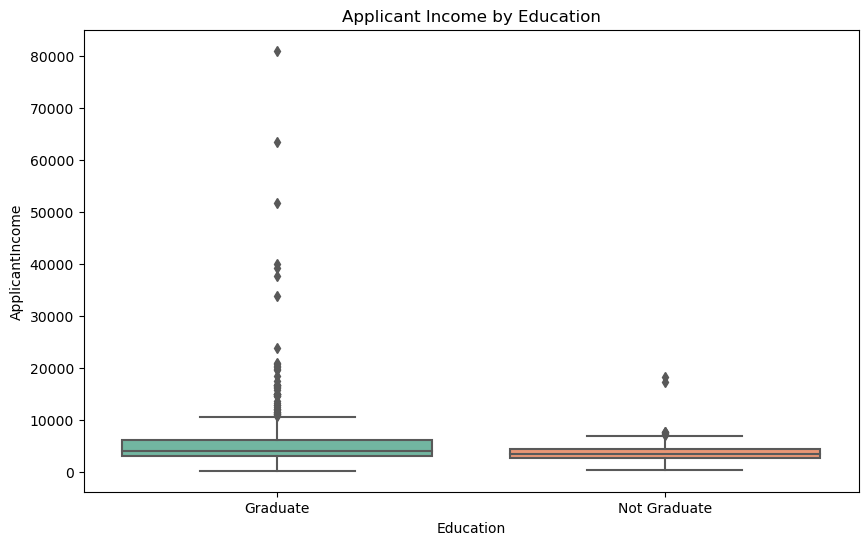
\includegraphics[width=15cm]{Applicant_Income_byEducation.png}
        \caption{Applicant Income by Education}
        \label{fig:sub1}
\end{center}
\end{figure}
\begin{figure}[H]
\begin{center}
        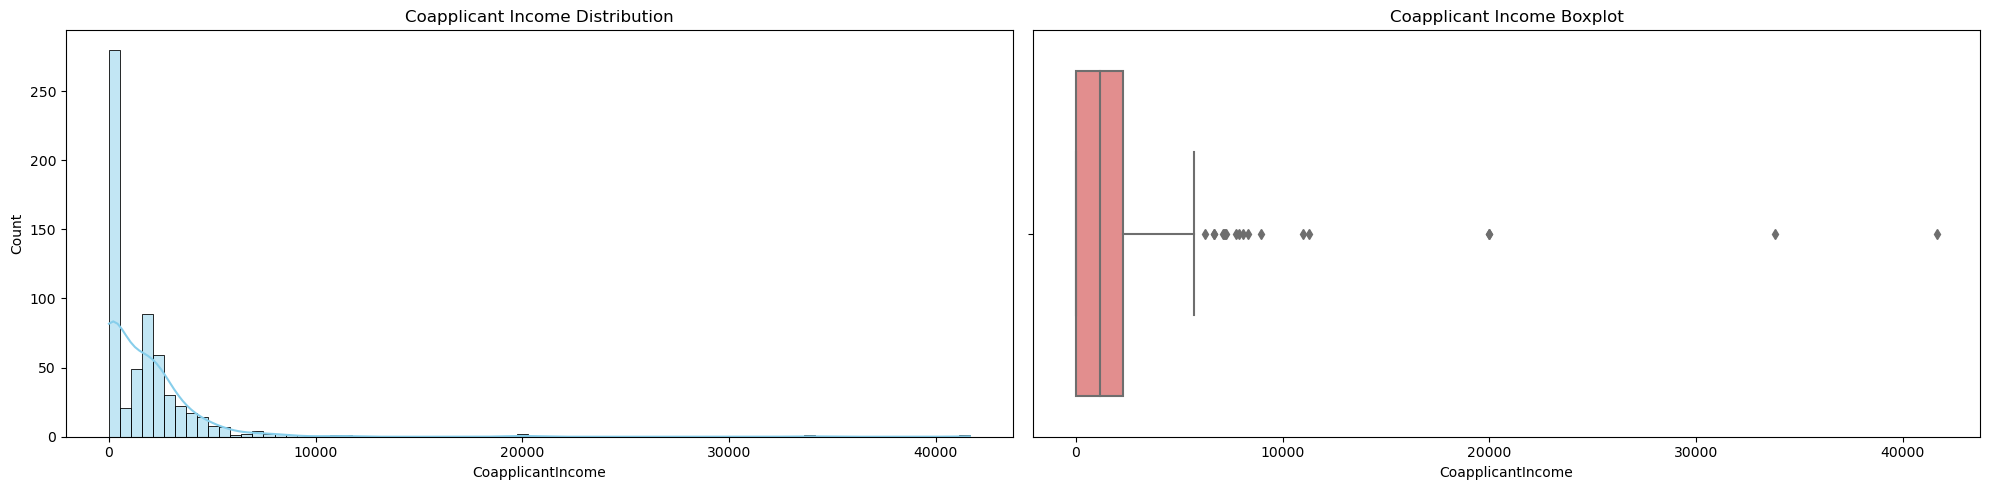
\includegraphics[width=15cm]{Coapplicant_income.png}
        \caption{Target Value: Coapplicant Income}
        \label{fig:sub1}
\end{center}
\end{figure}
\begin{figure}[H]
\begin{center}
        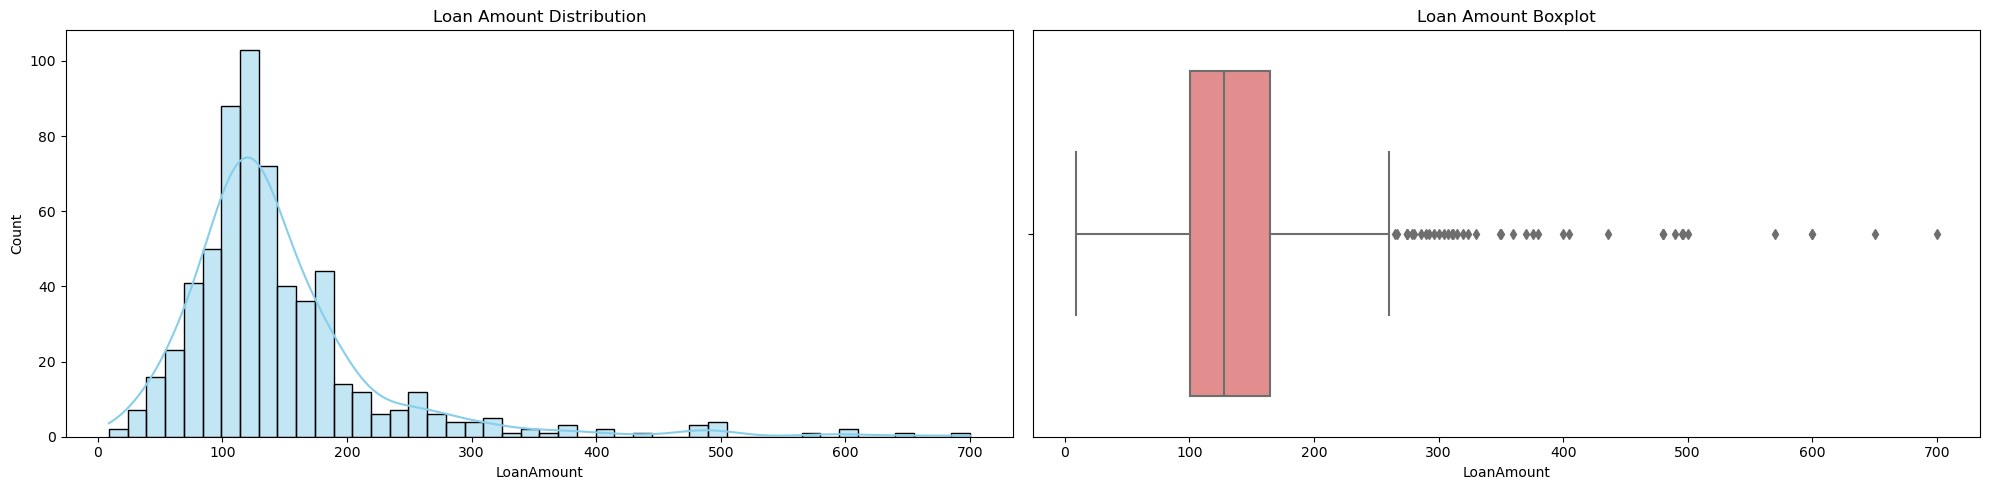
\includegraphics[width=15cm]{LoanAmount_Distribution.png}
        \caption{Target Value: Loan Amount}
        \label{fig:sub1}
\end{center}
\end{figure}

\subsection*{Bivariate Analysis}
\begin{figure}[H]
    \centering
    \begin{subfigure}[b]{0.45\linewidth}
        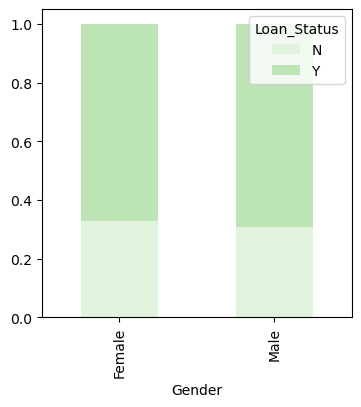
\includegraphics[width=\linewidth]{Gender_Bivariate.png}
        \caption{Target Value: Loan Status according to Gender}
        \label{fig:sub1}
    \end{subfigure}
    \hfill
    \begin{subfigure}[b]{0.45\linewidth}
        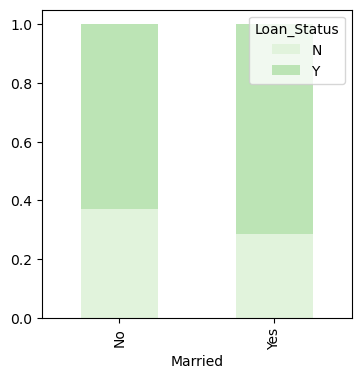
\includegraphics[width=\linewidth]{Marriage_Bivariate.png}
        \caption{Target Value: Loan Status according to Marriage}
        \label{fig:sub2}
    \end{subfigure}
    \begin{subfigure}[b]{0.45\linewidth}
        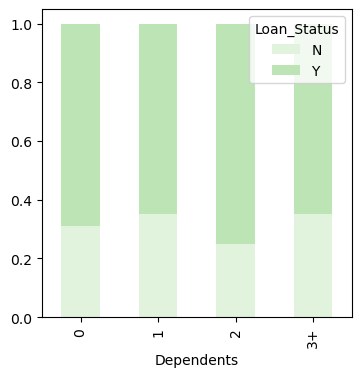
\includegraphics[width=\linewidth]{Dependents_Bivariate.png}
        \caption{Target Value: Loan Status according to Dependents}
        \label{fig:sub2}
    \end{subfigure}
    \begin{subfigure}[b]{0.45\linewidth}
        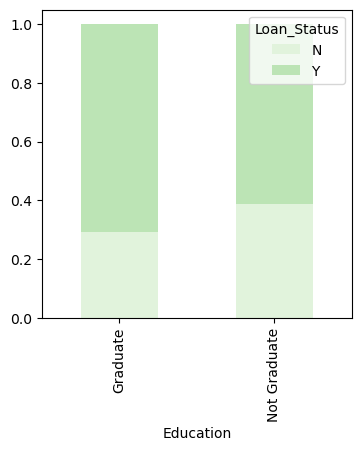
\includegraphics[width=\linewidth]{Education_Bivariate.png}
        \caption{Target Value: Loan Status according to Education}
        \label{fig:sub2}
    \end{subfigure}
    \caption{Bivariate Analysis for multiple attributes}
    \label{fig:panel}
\end{figure}
\begin{figure}[H]
    \centering
    \begin{subfigure}[b]{0.45\linewidth}
        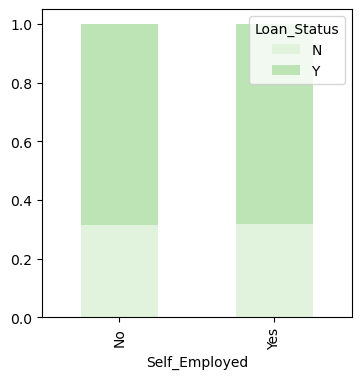
\includegraphics[width=\linewidth]{Employee_Bivariate.png}
        \caption{Target Value: Loan Status according to Employment}
        \label{fig:sub2}
    \end{subfigure}
    \begin{subfigure}[b]{0.45\linewidth}
        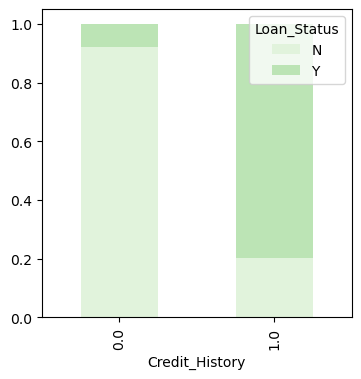
\includegraphics[width=\linewidth]{CreditHistory_Bivariate.png}
        \caption{Target Value: Loan Status according to Credit History}
        \label{fig:sub2}
    \end{subfigure}
    \caption{Bivariate Analysis for Employment and Credit History}
    \label{fig:panel}
\end{figure}
\begin{figure}[H]
    \centering
    \begin{subfigure}[b]{0.45\linewidth}
        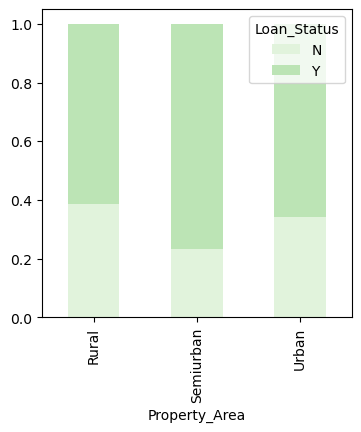
\includegraphics[width=\linewidth]{Property_Bivariate.png}
        \caption{Target Value: Loan Status according to Property Area}
        \label{fig:sub2}
    \end{subfigure}
    \begin{subfigure}[b]{0.45\linewidth}
        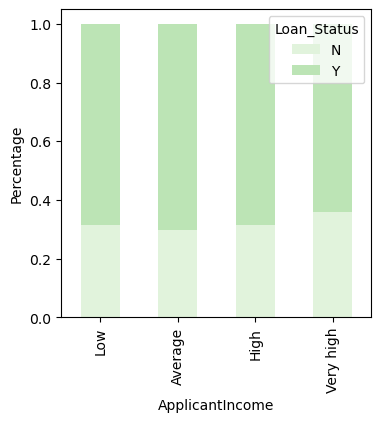
\includegraphics[width=\linewidth]{ApplicantIncome_Bivariate.png}
        \caption{Target Value: Loan Status according to Applicant Income}
        \label{fig:sub2}
    \end{subfigure}
    \caption{Bivariate Analysis for Property Area and Applicant Income}
    \label{fig:panel}
\end{figure}
\begin{figure}[H]
    \centering
    \begin{subfigure}[b]{0.45\linewidth}
        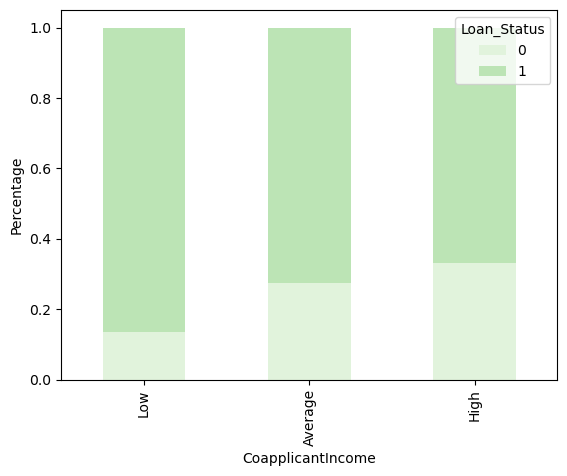
\includegraphics[width=\linewidth]{CoapplicantIncome_Bivariate.png}
        \caption{Target Value: Loan Status according to Coapplicant Income}
        \label{fig:sub2}
    \end{subfigure}
    \begin{subfigure}[b]{0.45\linewidth}
        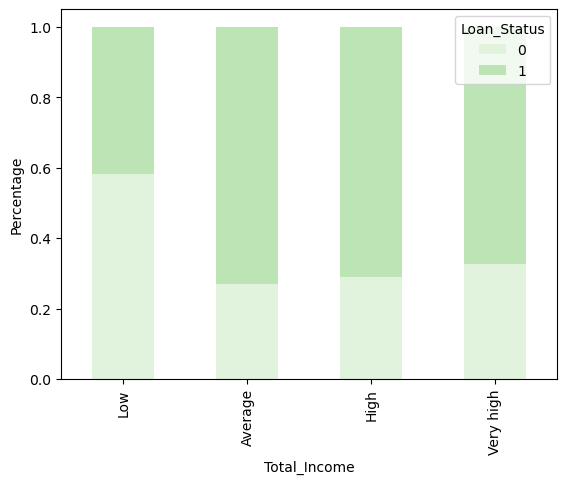
\includegraphics[width=\linewidth]{TotalIncome_Bivariate.png}
        \caption{Target Value: Loan Status according to Total Income}
        \label{fig:sub2}
    \end{subfigure}
    \caption{Bivariate Analysis for Coapplicant Income and Total Income}
    \label{fig:panel}
\end{figure}
\begin{figure}[H]
\begin{center}
        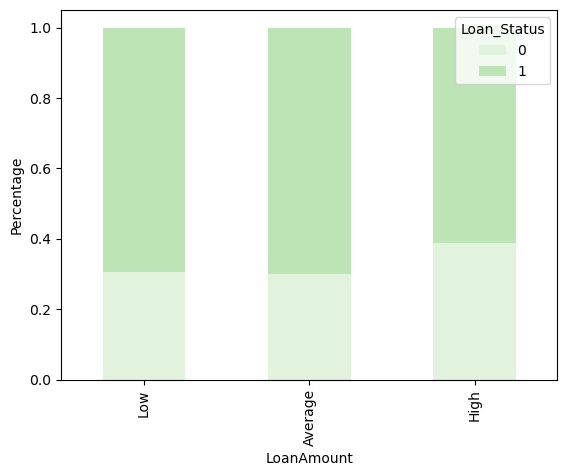
\includegraphics[width=0.5\linewidth]{LoanAmount_Bivariate.png}
        \caption{Target Value: Loan Status according to Loan Amount}
        \label{fig:sub1}
\end{center}
\end{figure}

\subsection*{Correlation Using HeatMap}
\begin{figure}[H]
\begin{center}
        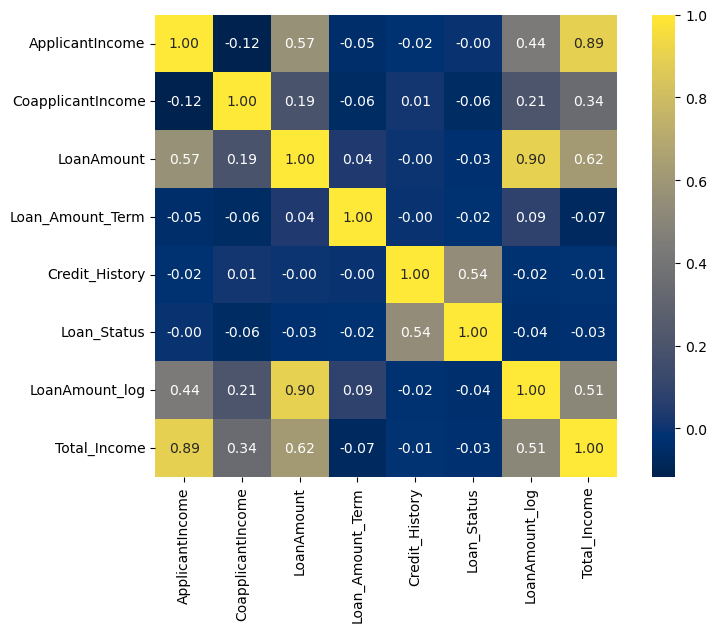
\includegraphics[width=\linewidth]{Correlation_plot.png}
        \caption{Correlation Matrix for numeric attributes}
        \label{fig:sub1}
\end{center}
\end{figure}

    \item \textbf{Data Preprocessing:} Clean and prepare the data for analysis by handling missing values, dropping unwanted columns which will not be used for further analysis.
    \subsection*{Outlier Treatment}
            \begin{figure}[H]
            \begin{center}
                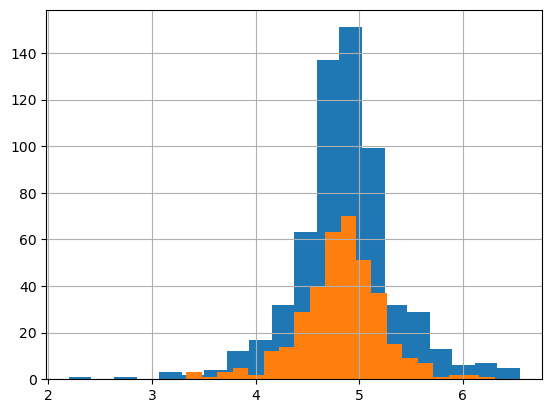
\includegraphics[width=\linewidth]{Outlier_treatment.png}
                \caption{Outlier Treatment for training and testing set}
                \label{fig:sub1}
            \end{center}
            \end{figure}
    \item \textbf{Feature Selection:} Identify the most relevant features that significantly impact loan approval and default rates.
    
    \item \textbf{Model Training:} Develop and train machine learning models (Logistic Regression, Decision Trees, K-Means Clustering) using historical data to predict loan approval outcomes.
\begin{figure}[H]
\begin{center}
        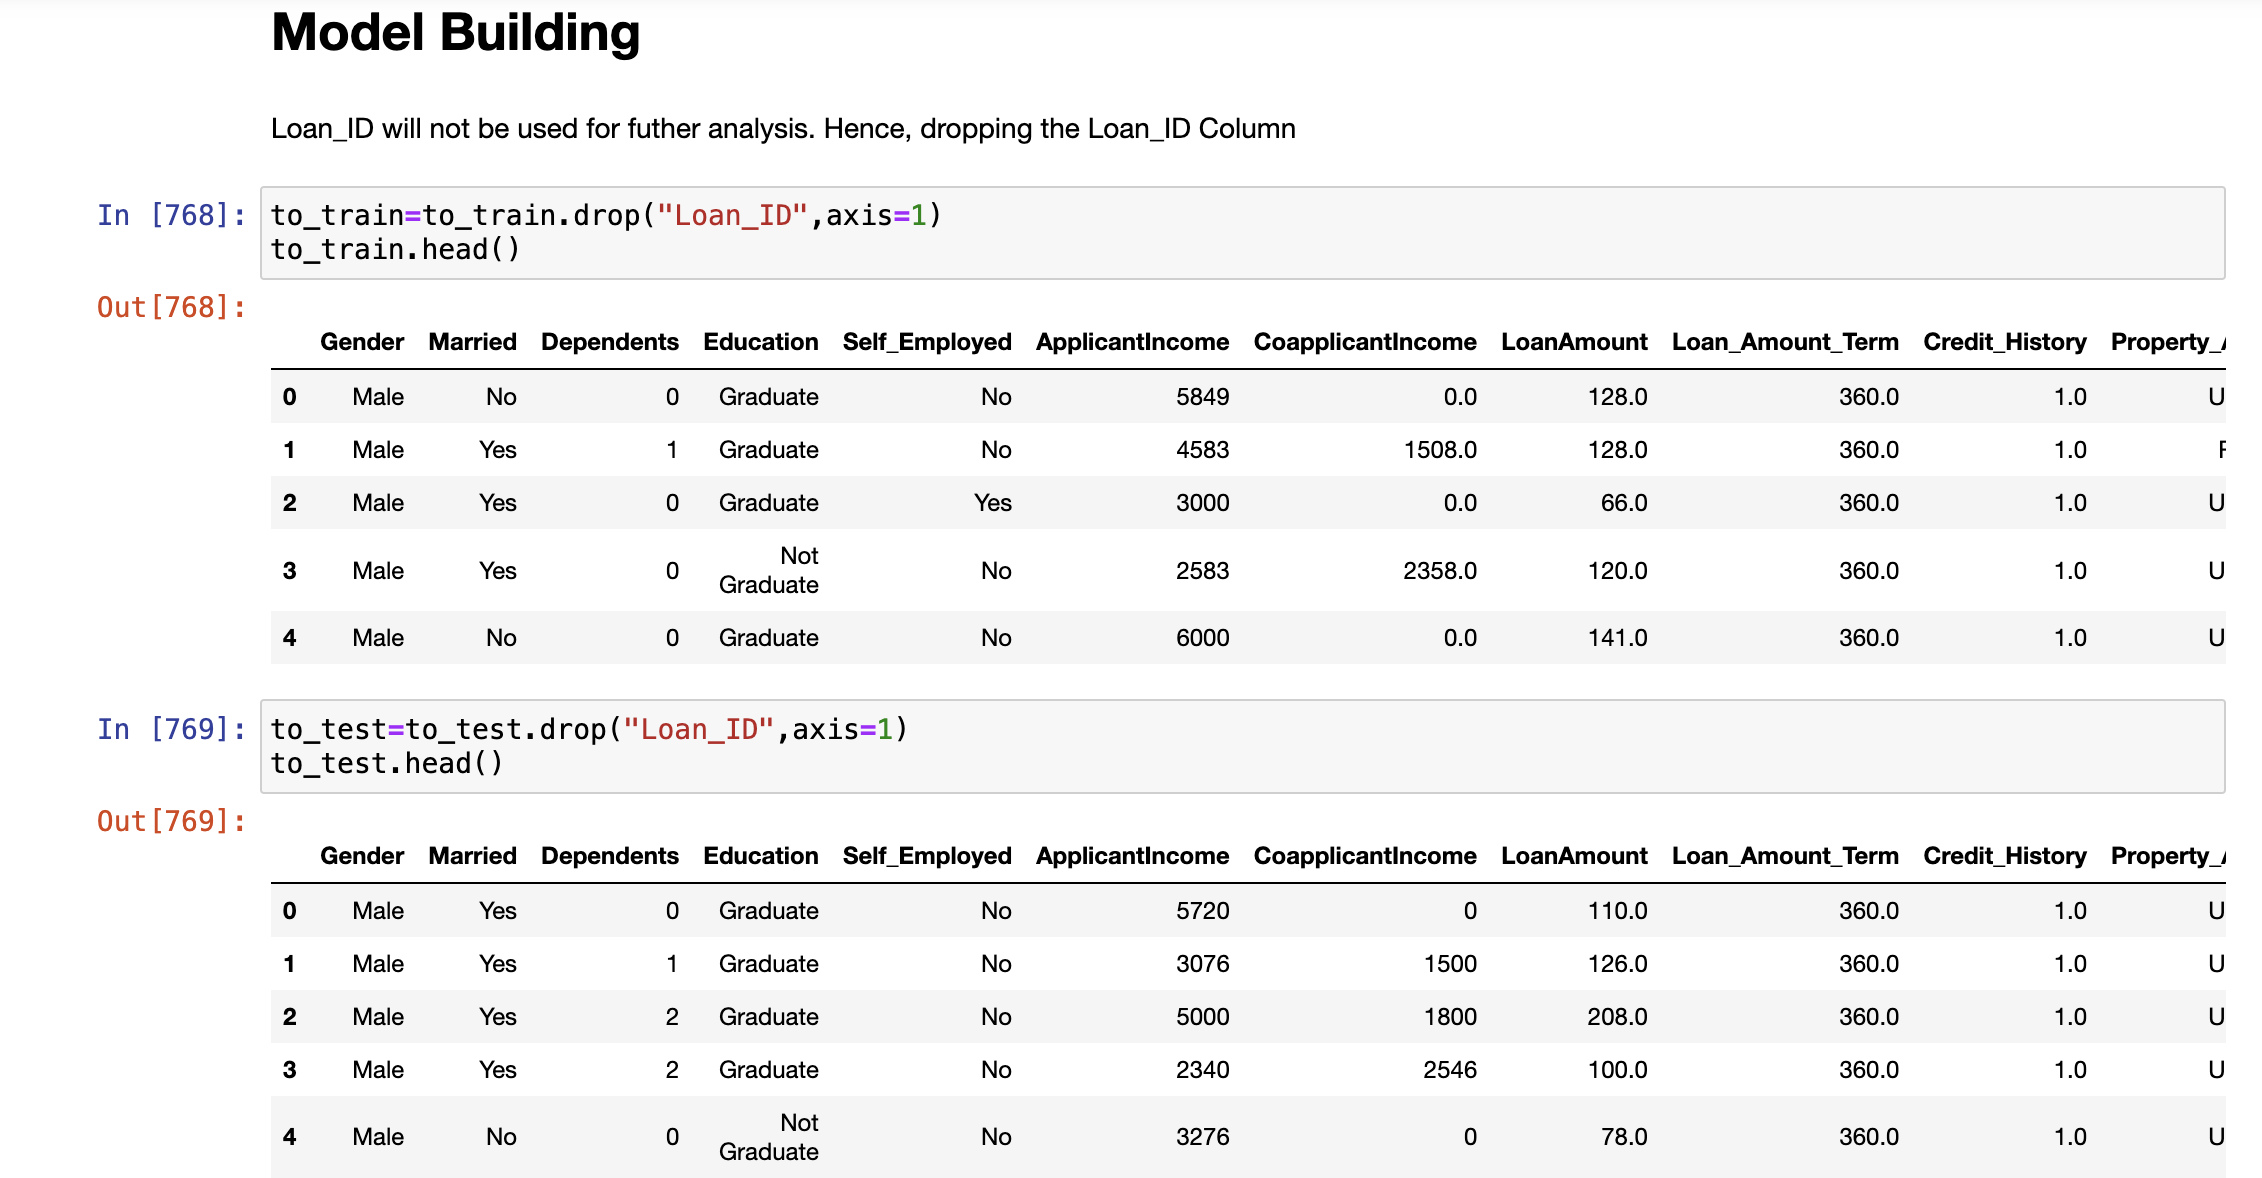
\includegraphics[width=\linewidth]{Model_Building_1.png}
        \label{fig:sub1}
\end{center}
\end{figure}
\begin{figure}[H]
\begin{center}
        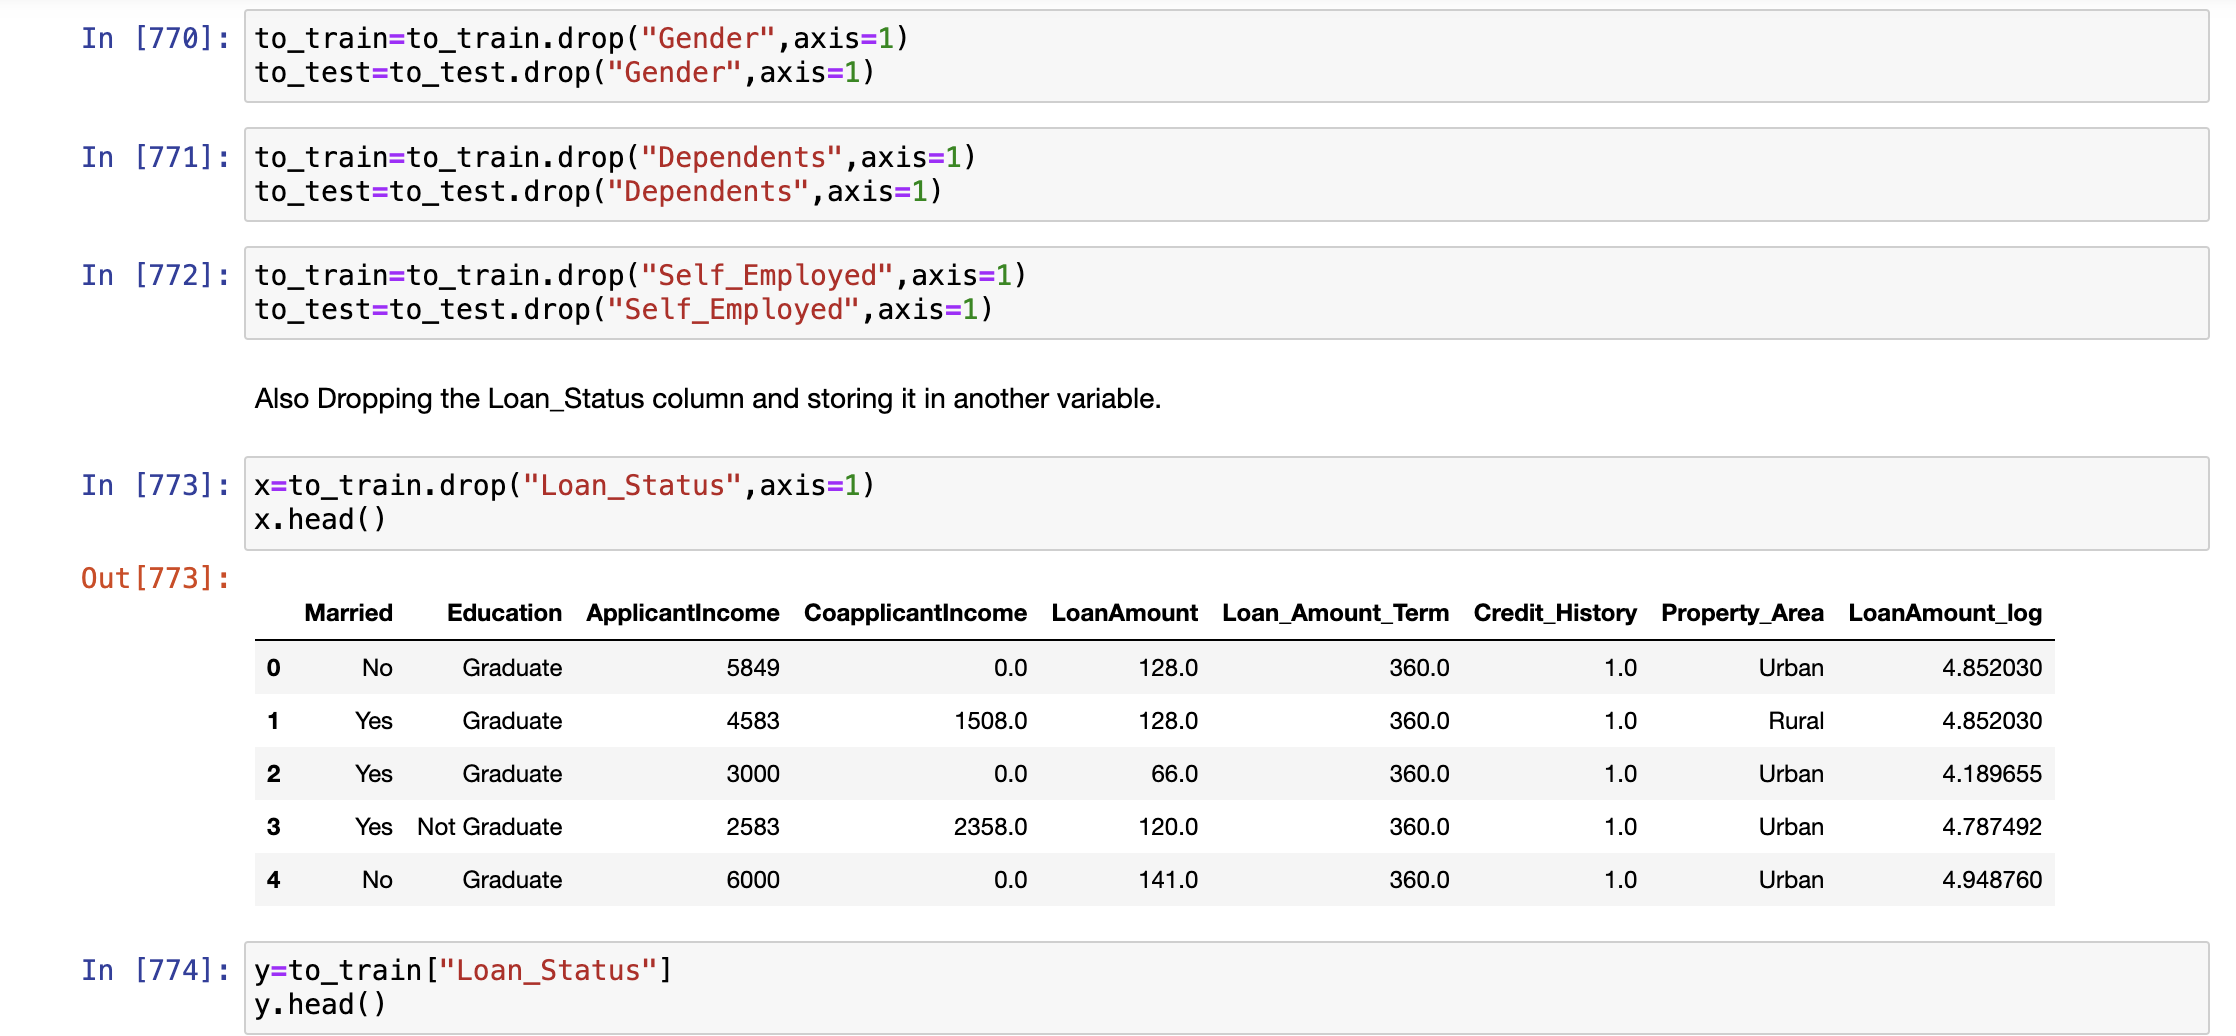
\includegraphics[width=\linewidth]{Model_Building_2.png}
        \label{fig:sub1}
\end{center}
\end{figure}
\begin{figure}[H]
\begin{center}
        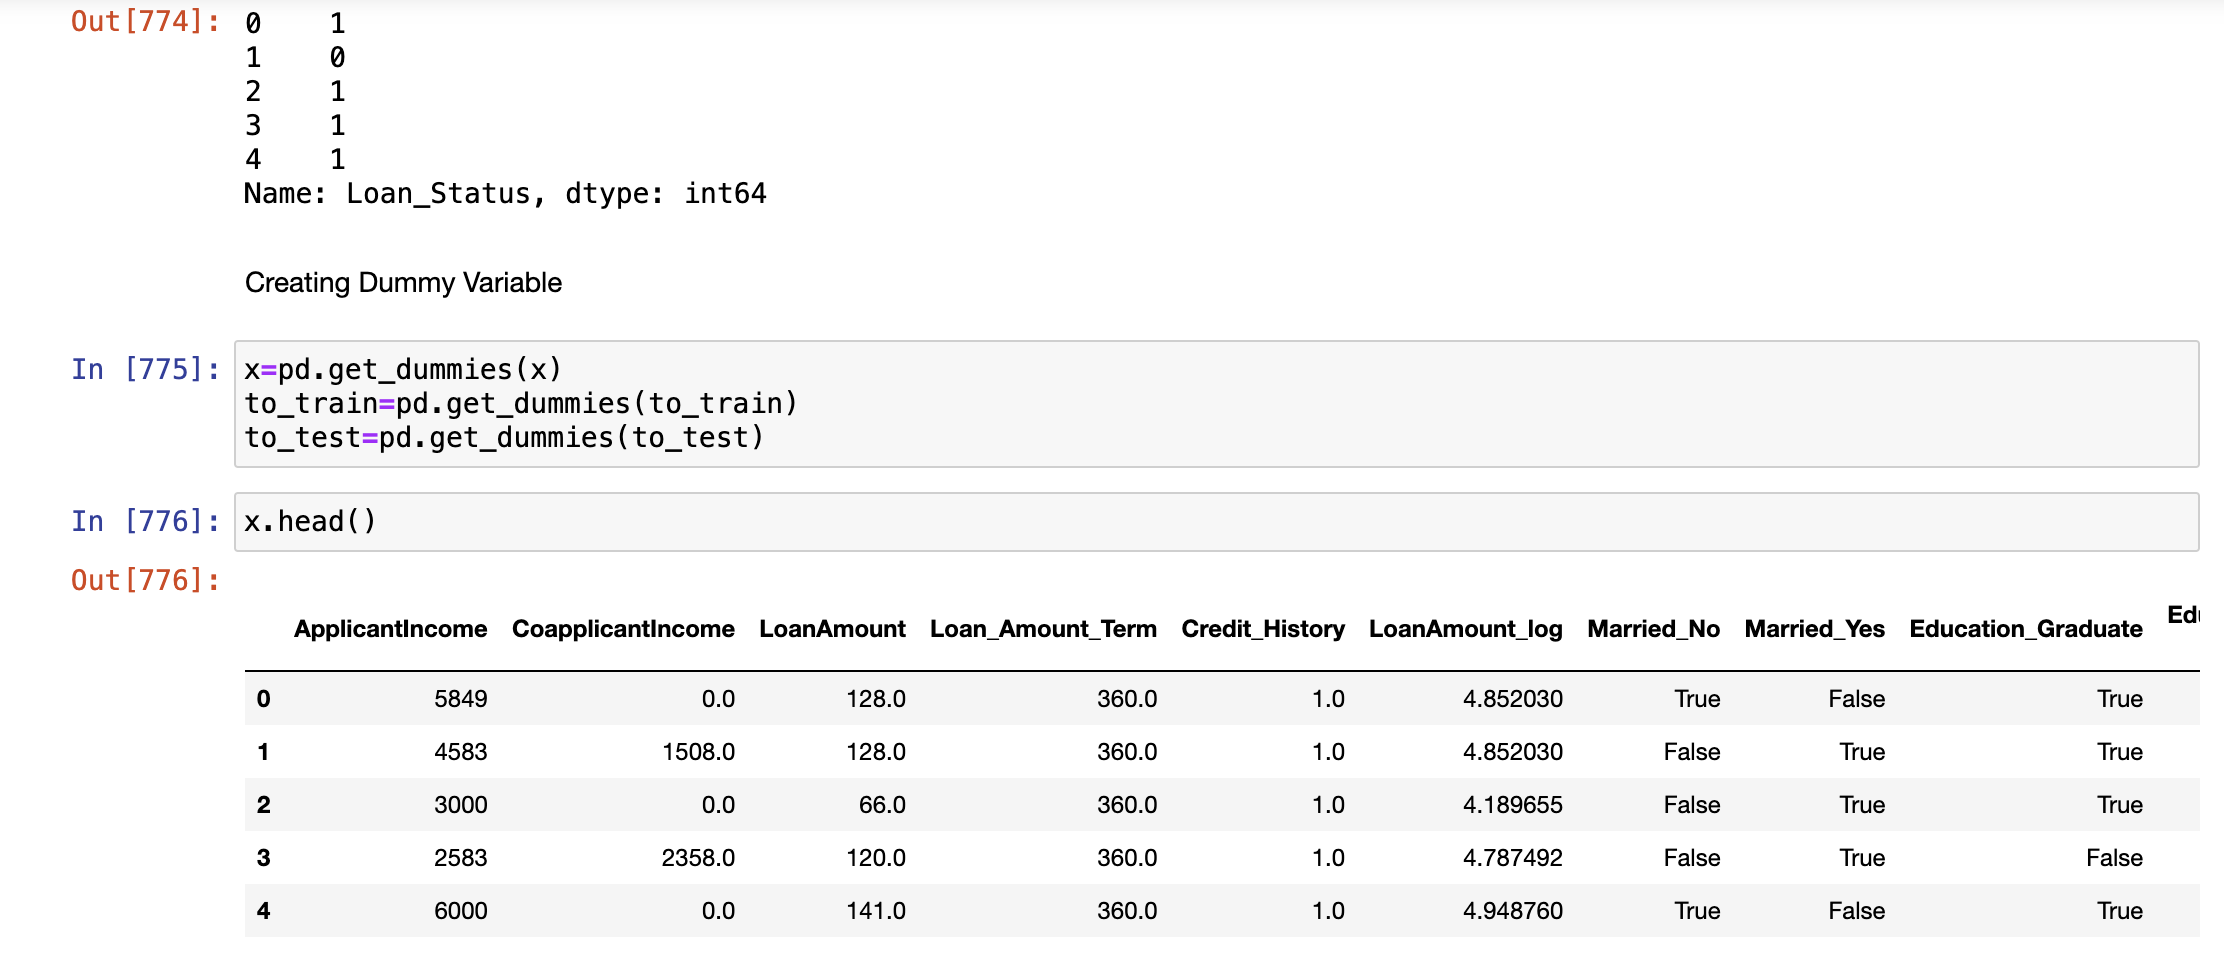
\includegraphics[width=\linewidth]{Model_Building_3.png}
        \label{fig:sub1}
\end{center}
\end{figure}
    
    \item \textbf{Model Evaluation:} Assess the performance of trained models using  accuracy metrics to ensure reliability of predictions.
\begin{figure}[H]
\begin{center}
        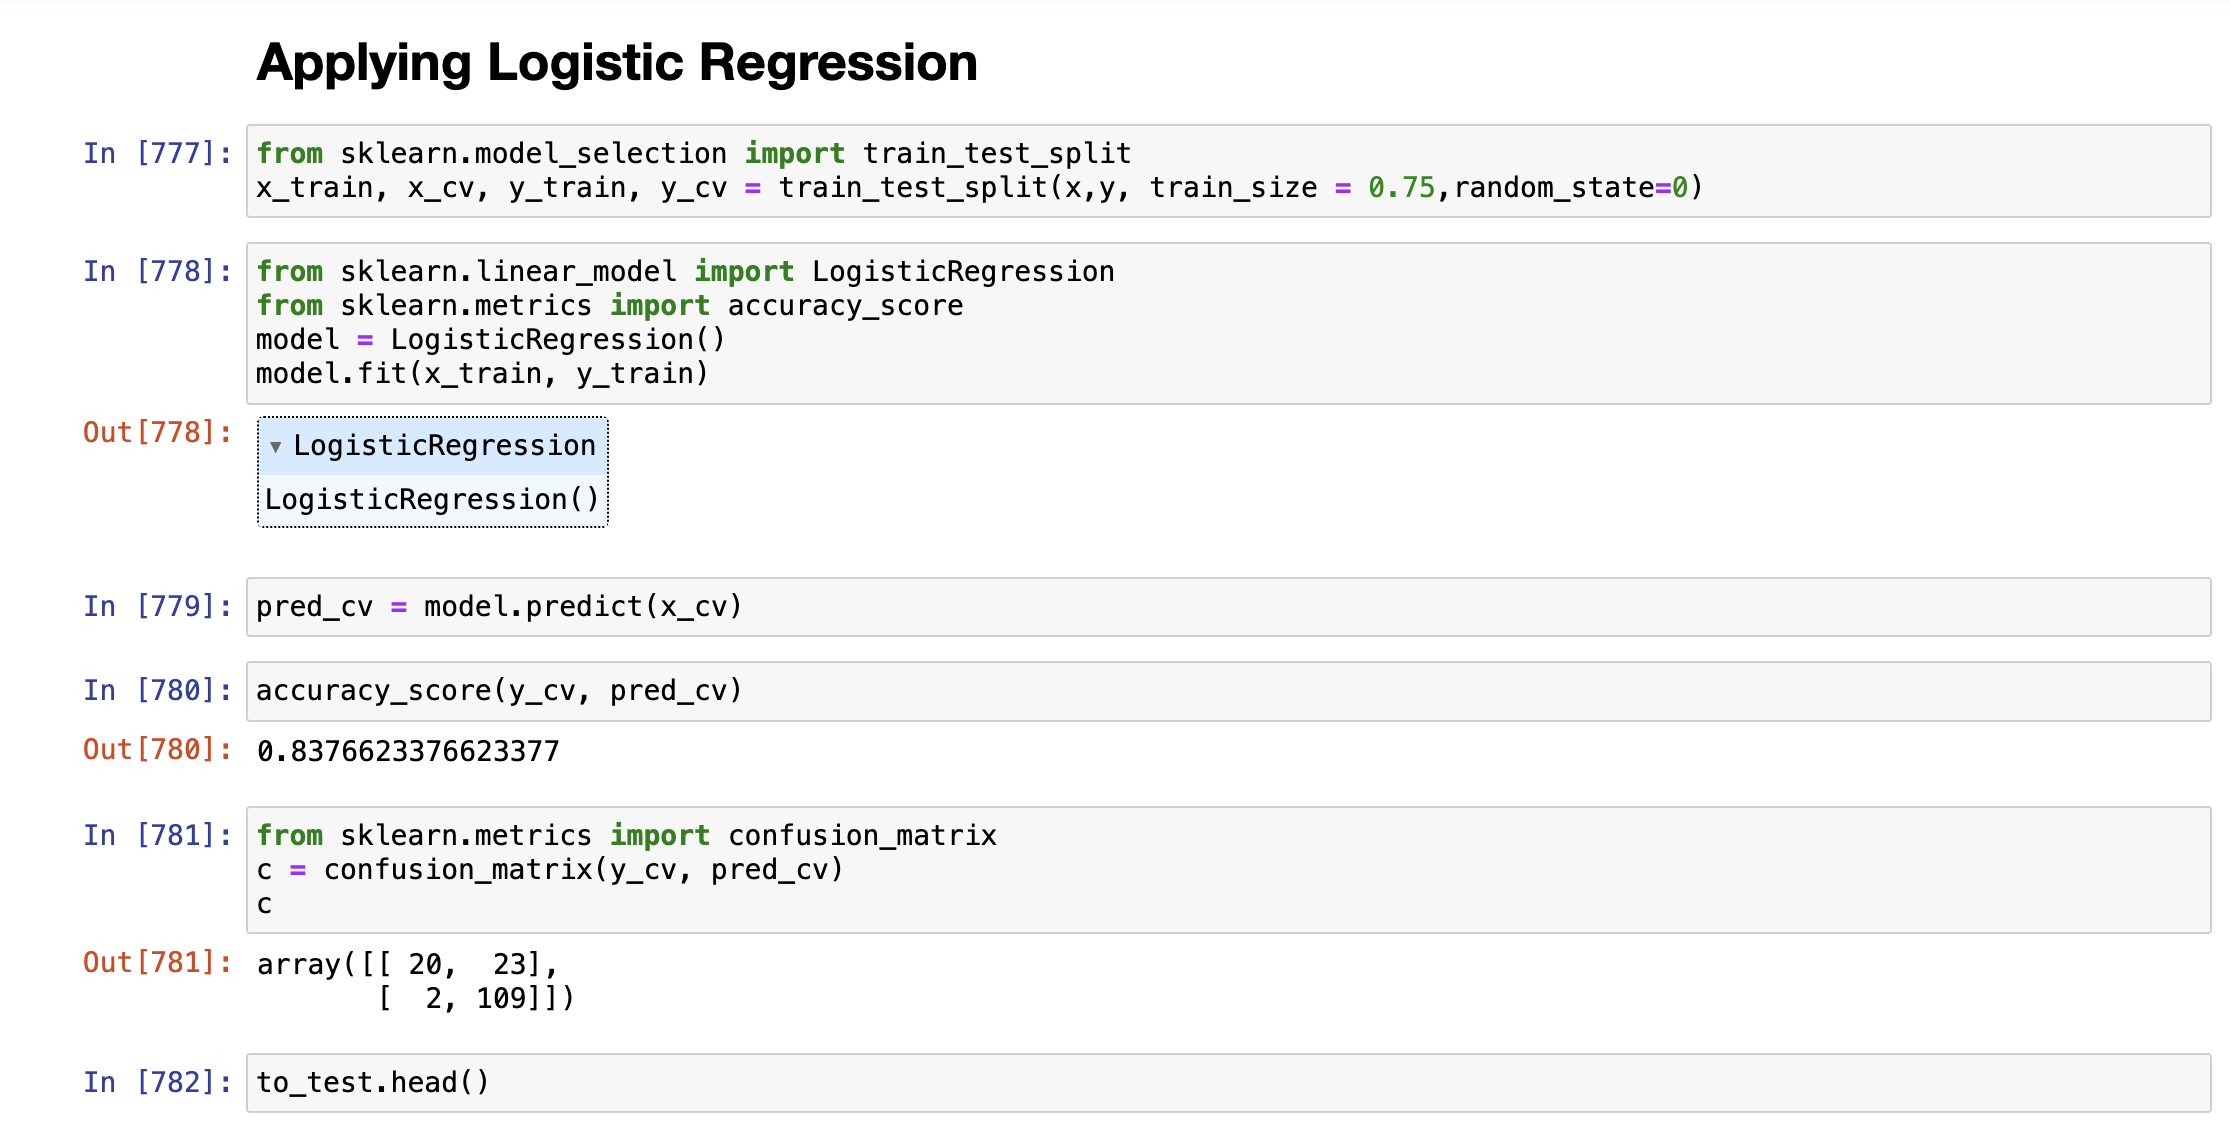
\includegraphics[width=\linewidth]{Applying_LR_1.png}
        \label{fig:sub1}
\end{center}
\end{figure}
\begin{figure}[H]
\begin{center}
        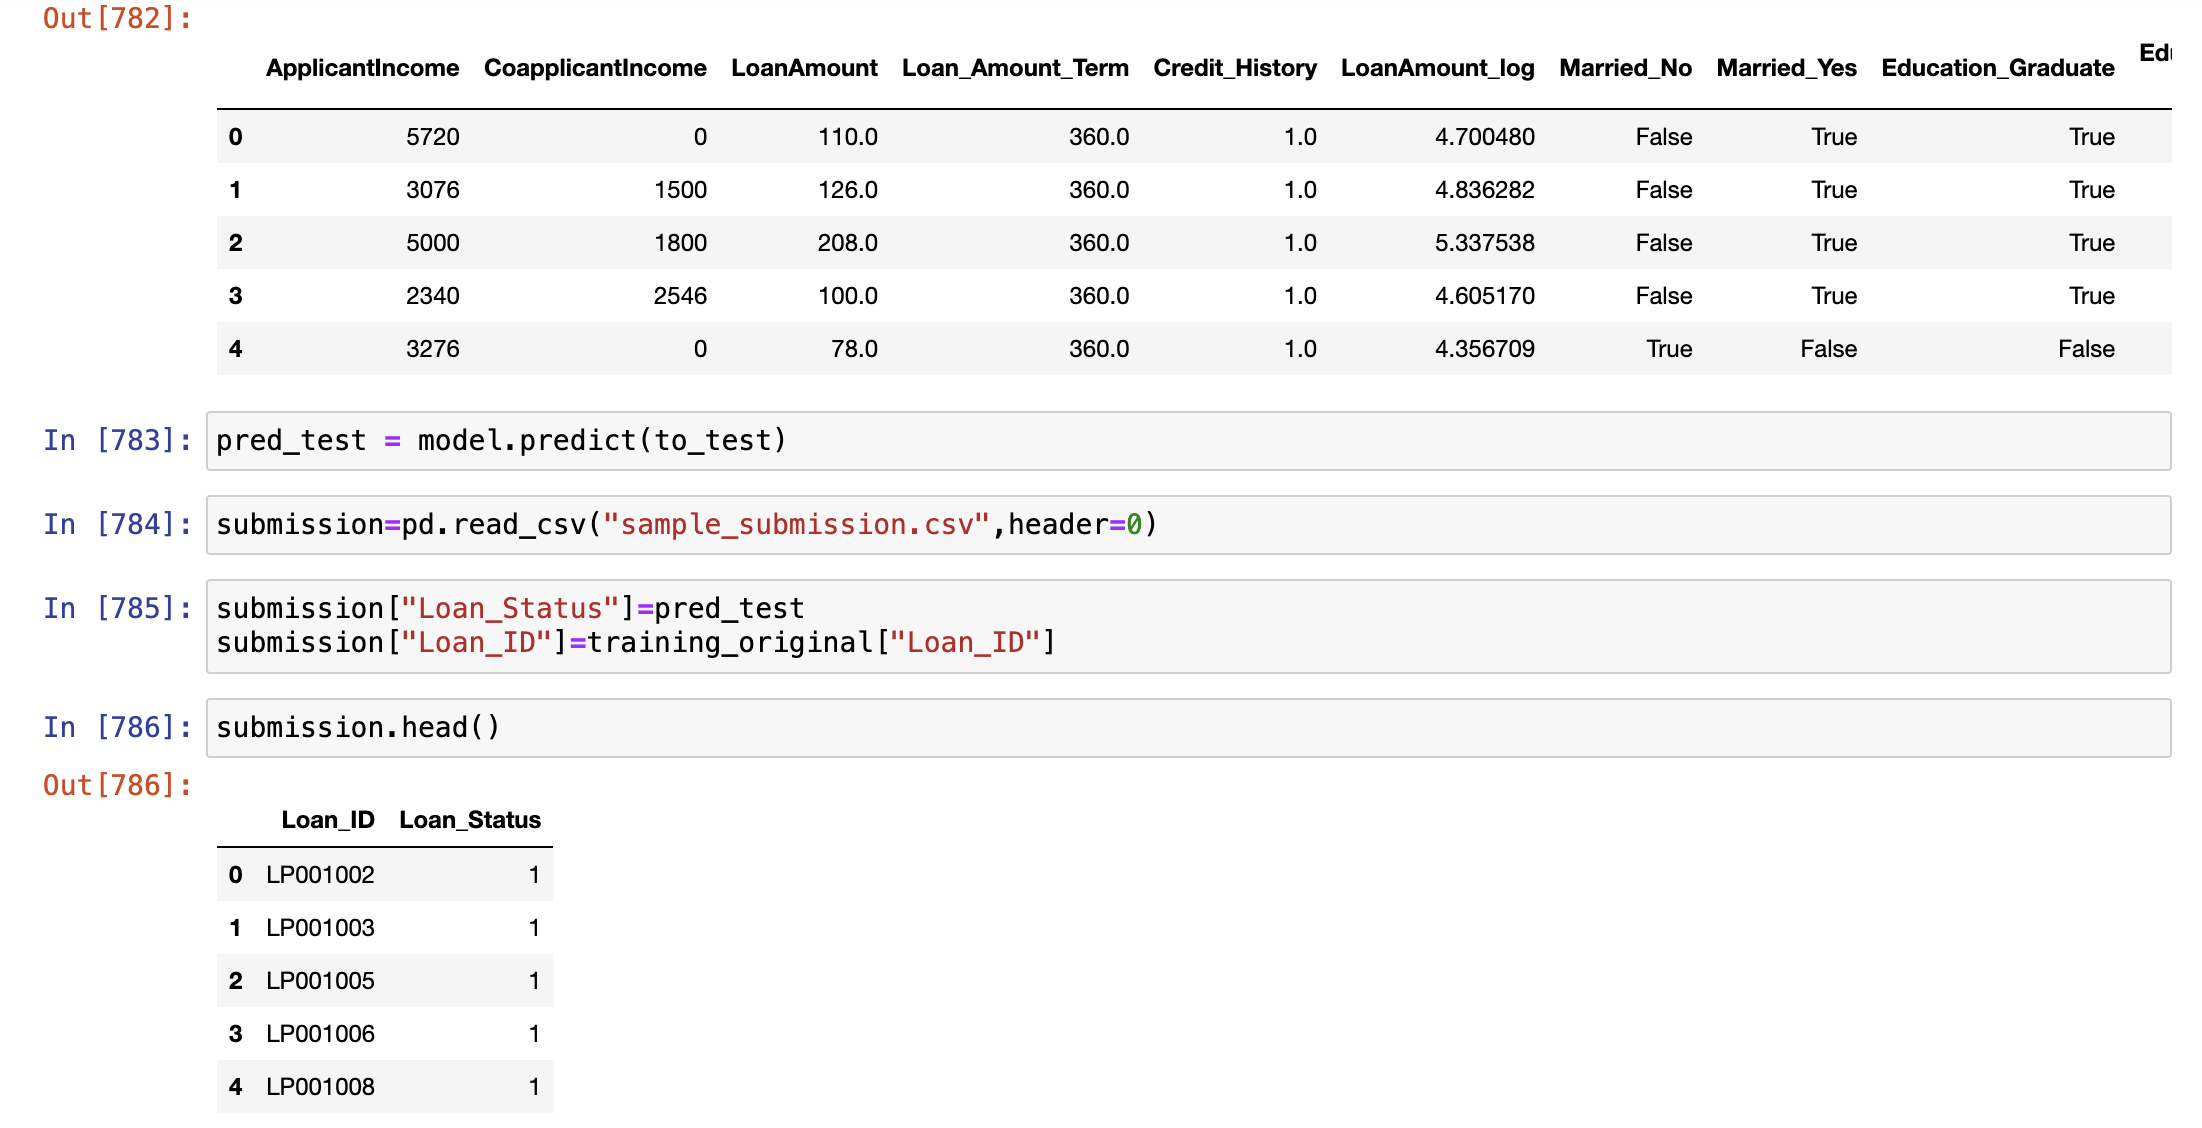
\includegraphics[width=\linewidth]{Applying_LR_2.png}
        \label{fig:sub1}
\end{center}
\end{figure}
\begin{figure}[H]
\begin{center}
        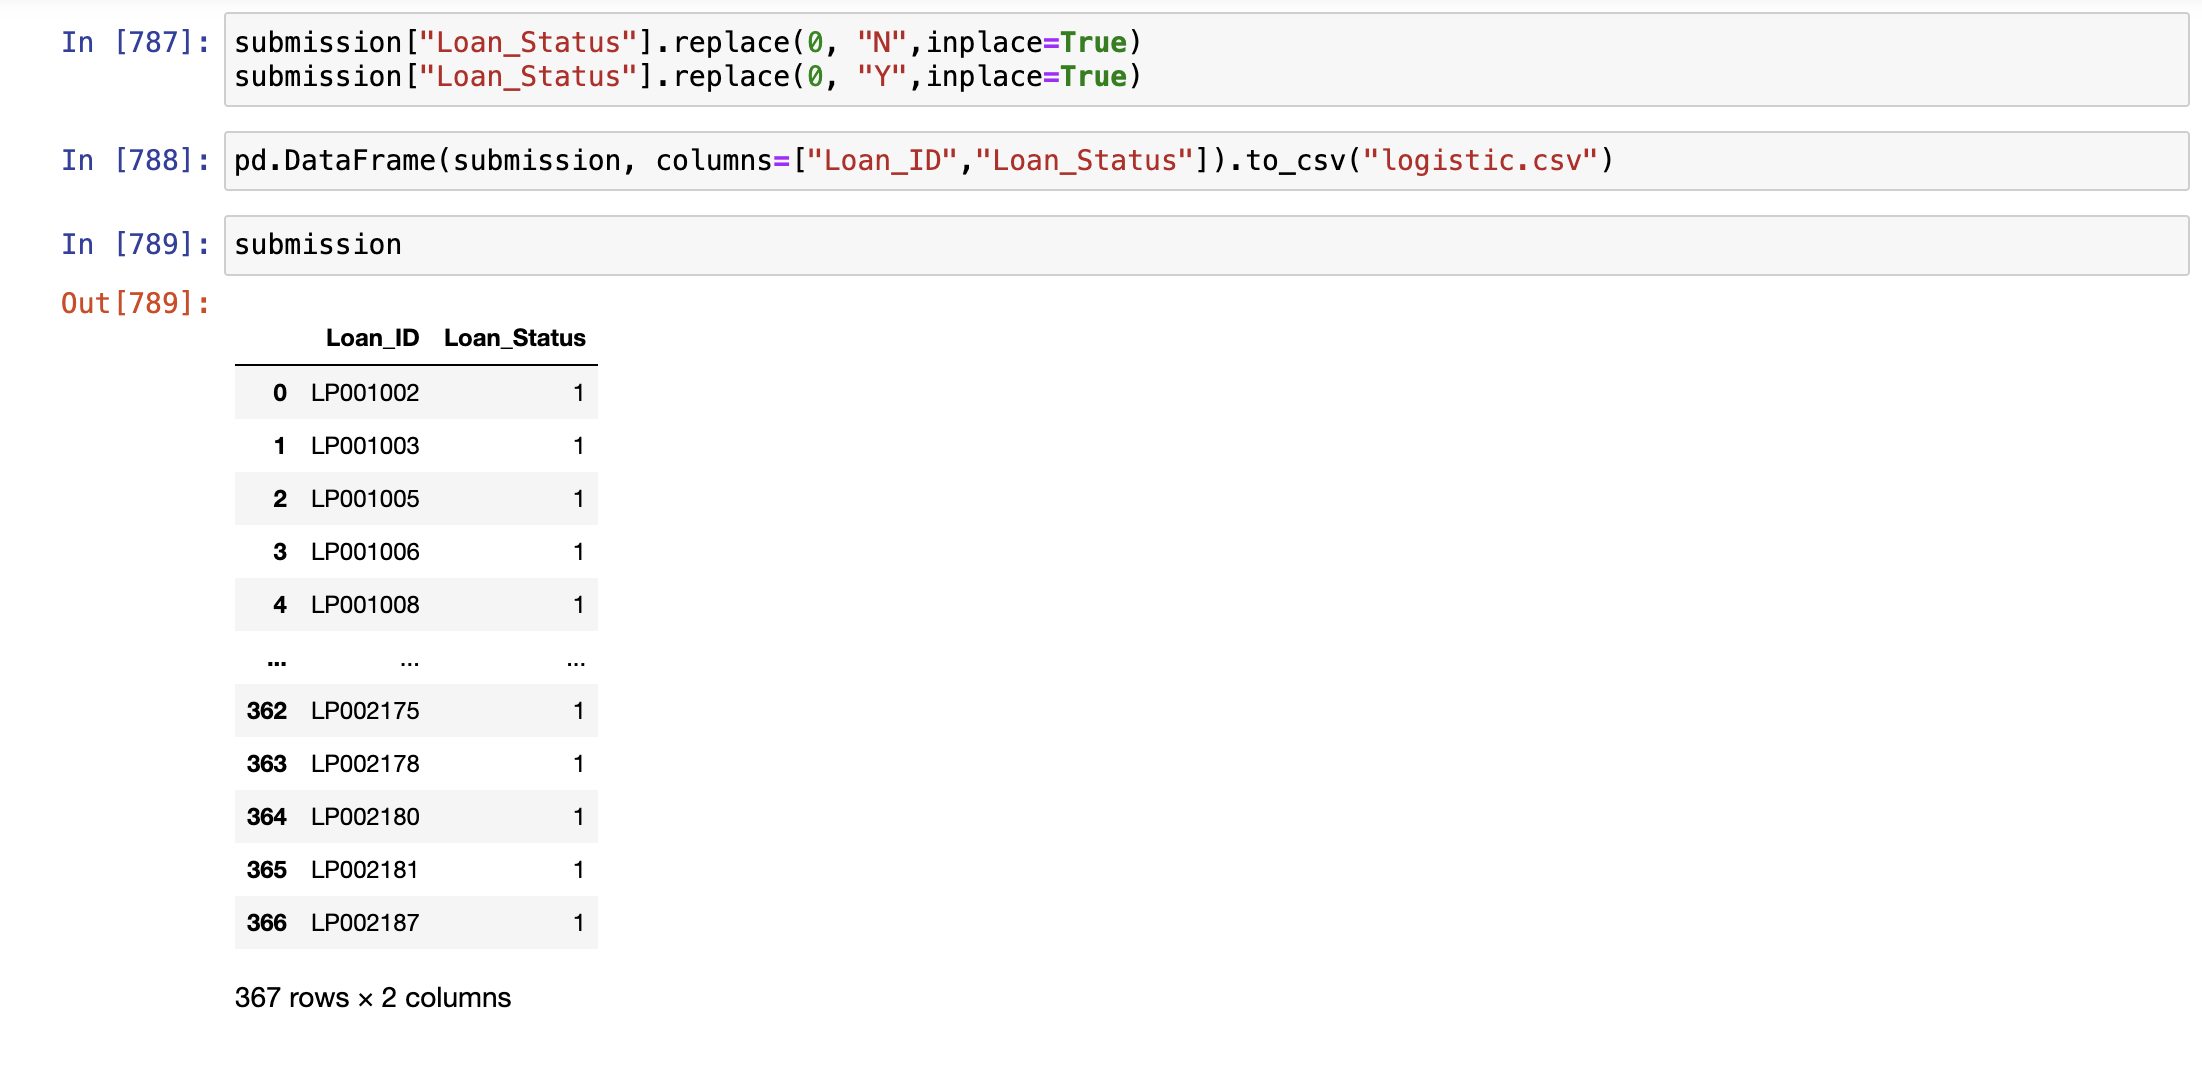
\includegraphics[width=\linewidth]{Applying_LR_3.png}
        \label{fig:sub1}
\end{center}
\end{figure}
\begin{figure}[H]
\begin{center}
        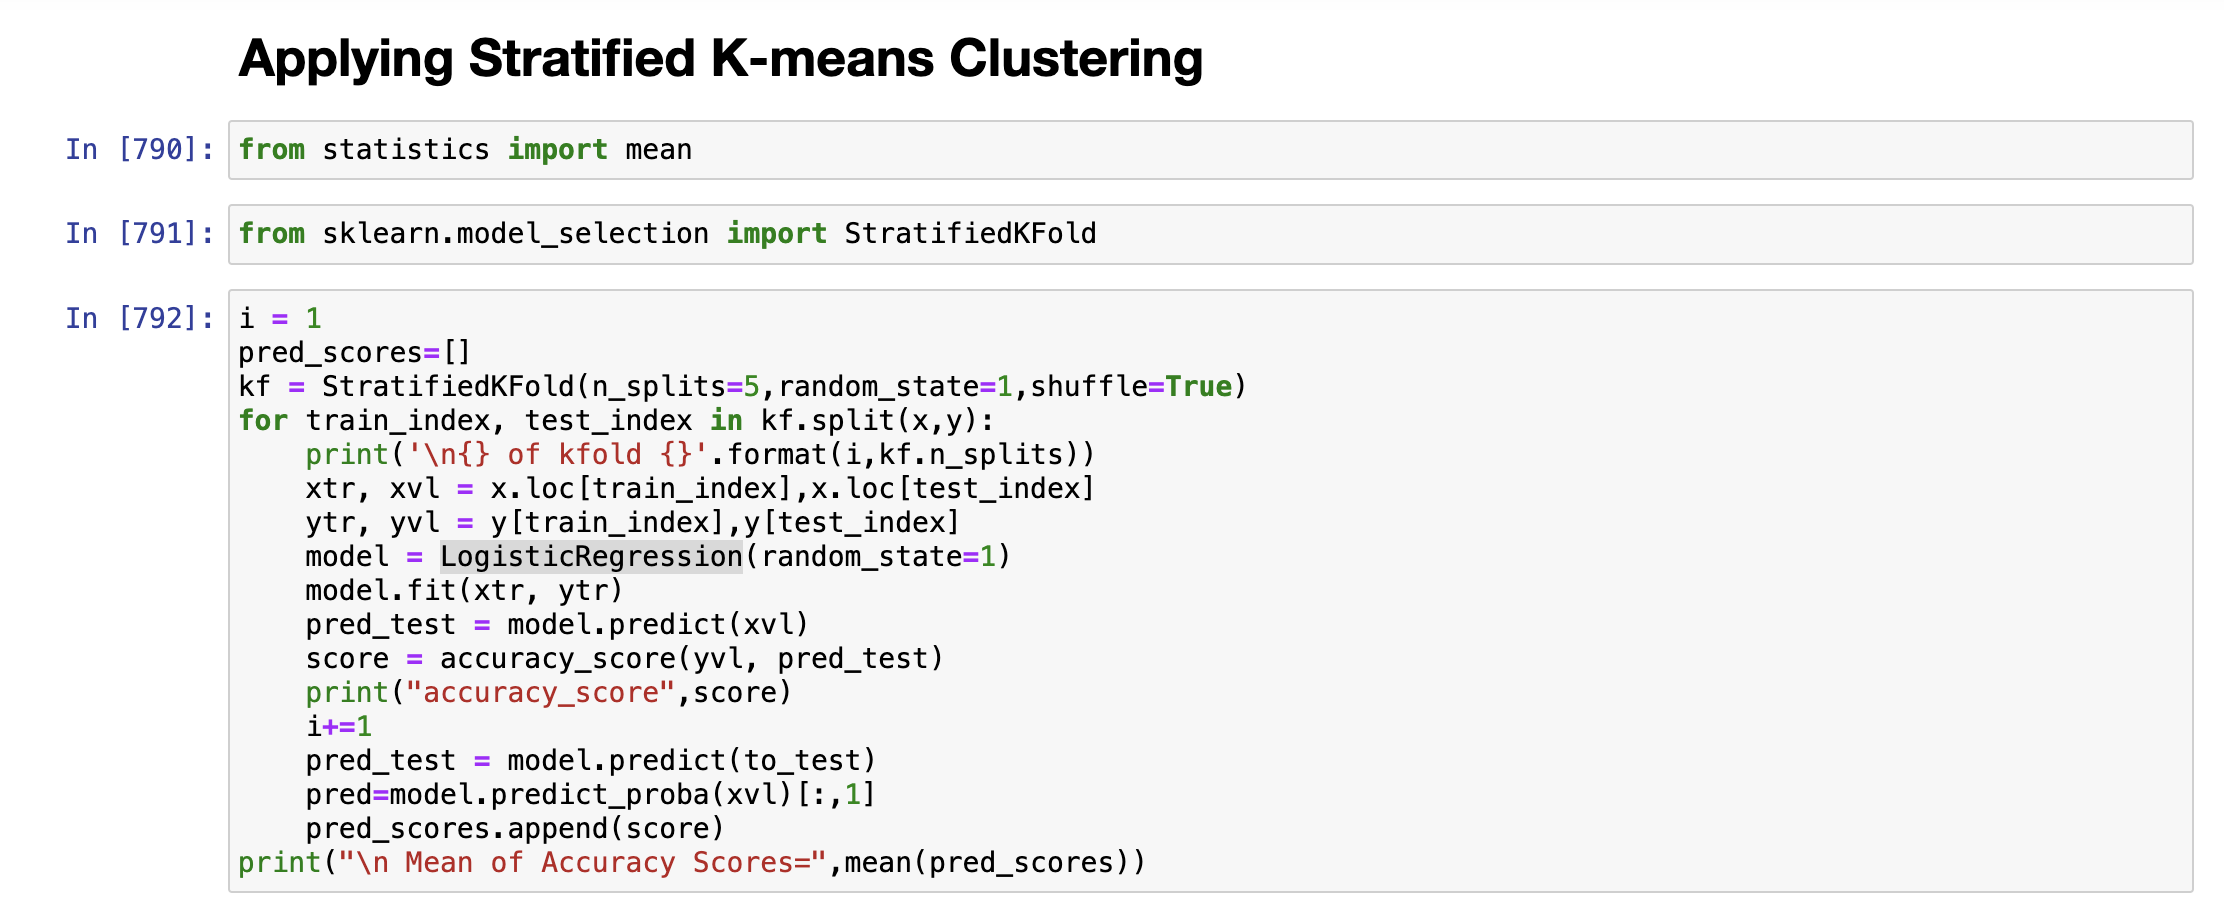
\includegraphics[width=\linewidth]{Applying_K-means_1.png}
        \label{fig:sub1}
\end{center}
\end{figure}
\begin{figure}[H]
\begin{center}
        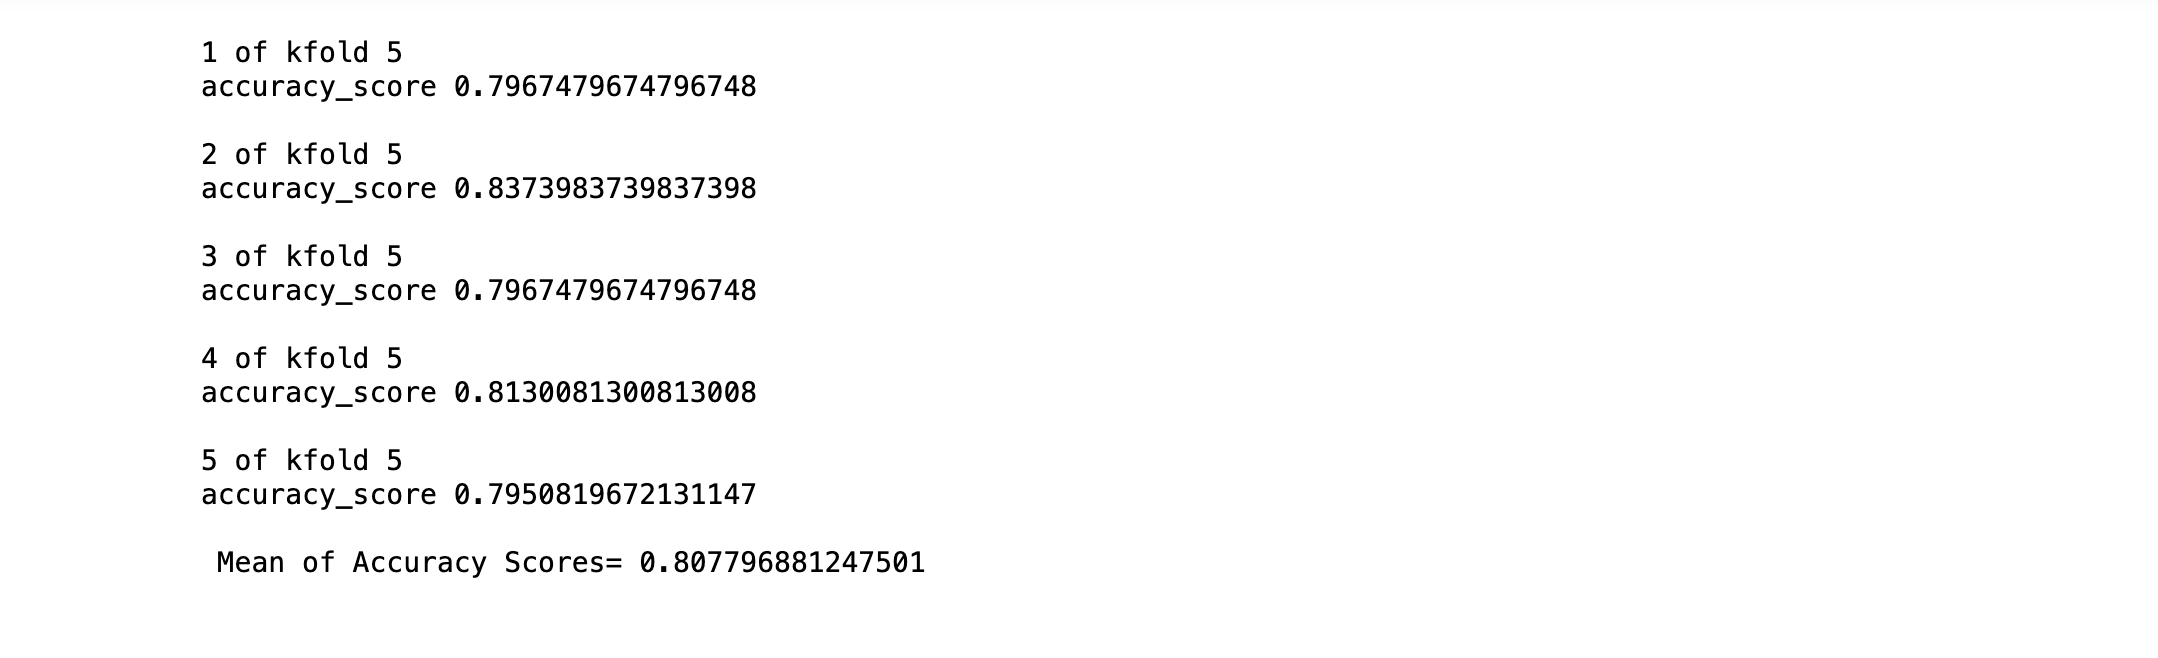
\includegraphics[width=\linewidth]{Applying_K-means_2.png}
        \label{fig:sub1}
\end{center}
\end{figure}
\begin{figure}[H]
\begin{center}
        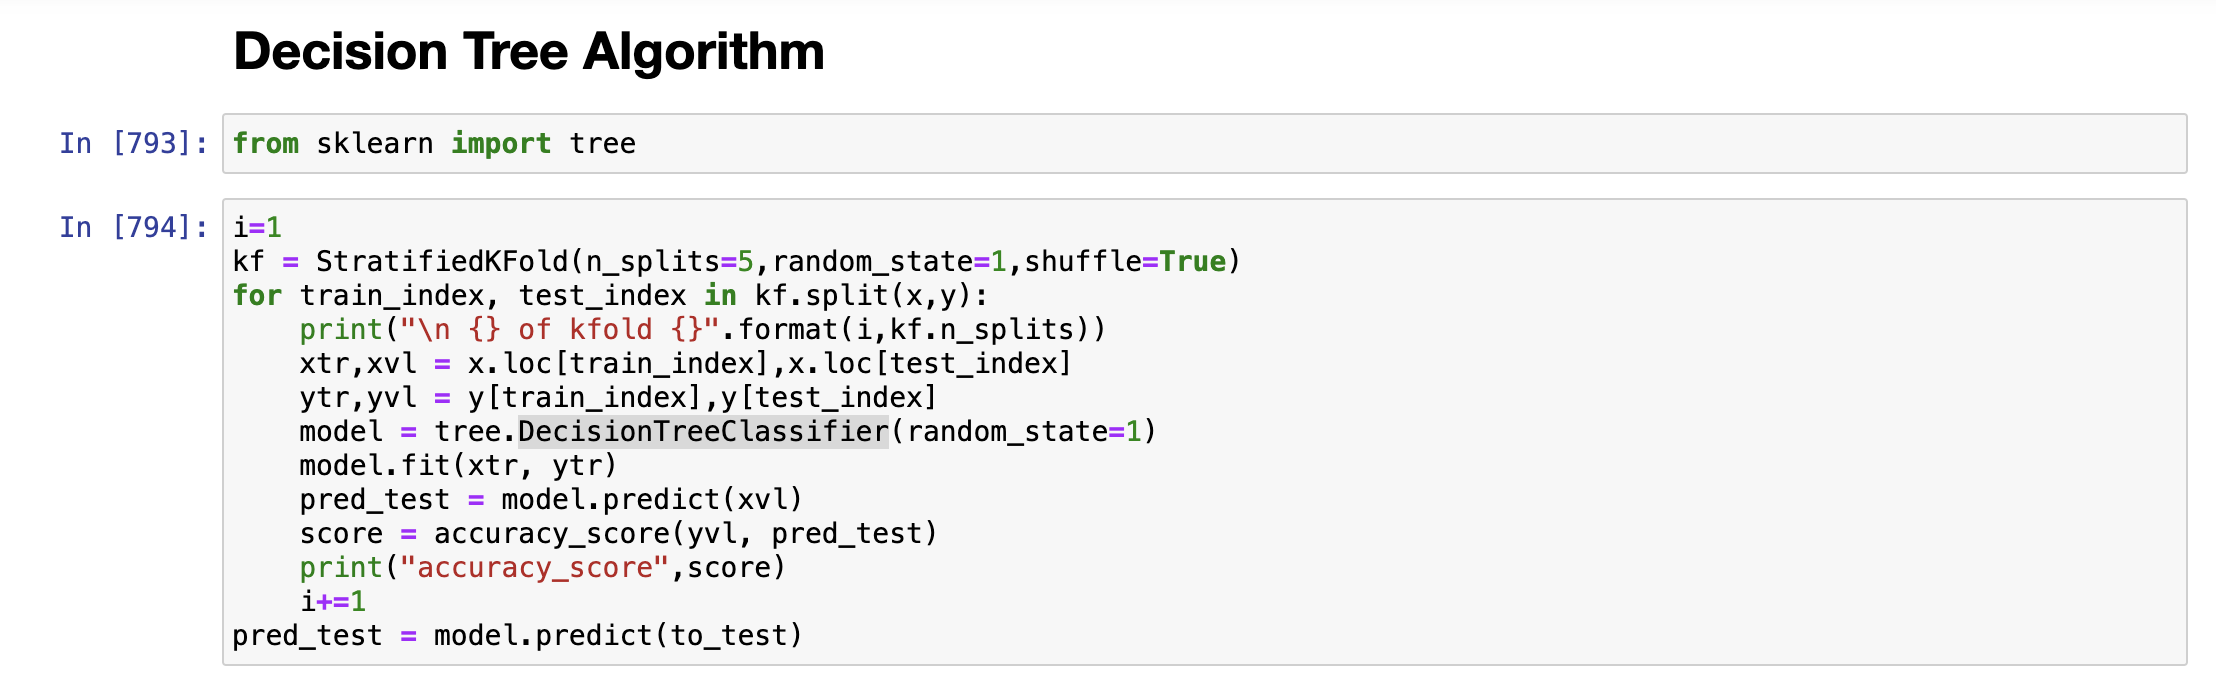
\includegraphics[width=\linewidth]{Decision_Tree_1.png}
        \label{fig:sub1}
\end{center}
\end{figure}
\begin{figure}[H]
\begin{center}
        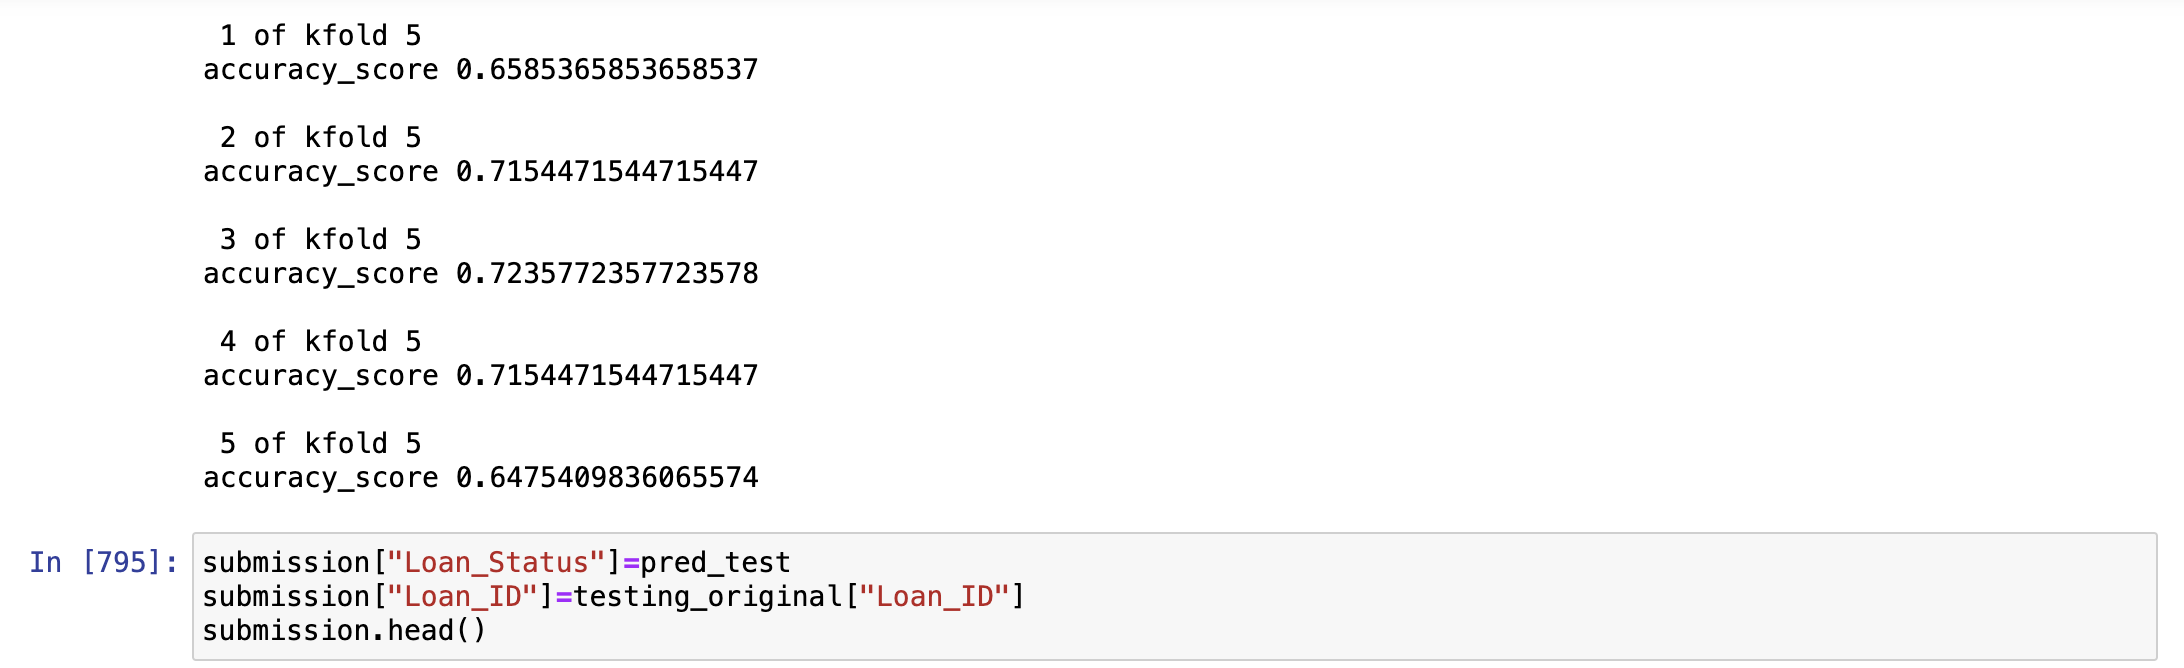
\includegraphics[width=\linewidth]{Decision_Tree_2.png}
        \label{fig:sub1}
\end{center}
\end{figure}
\begin{figure}[H]
\begin{center}
        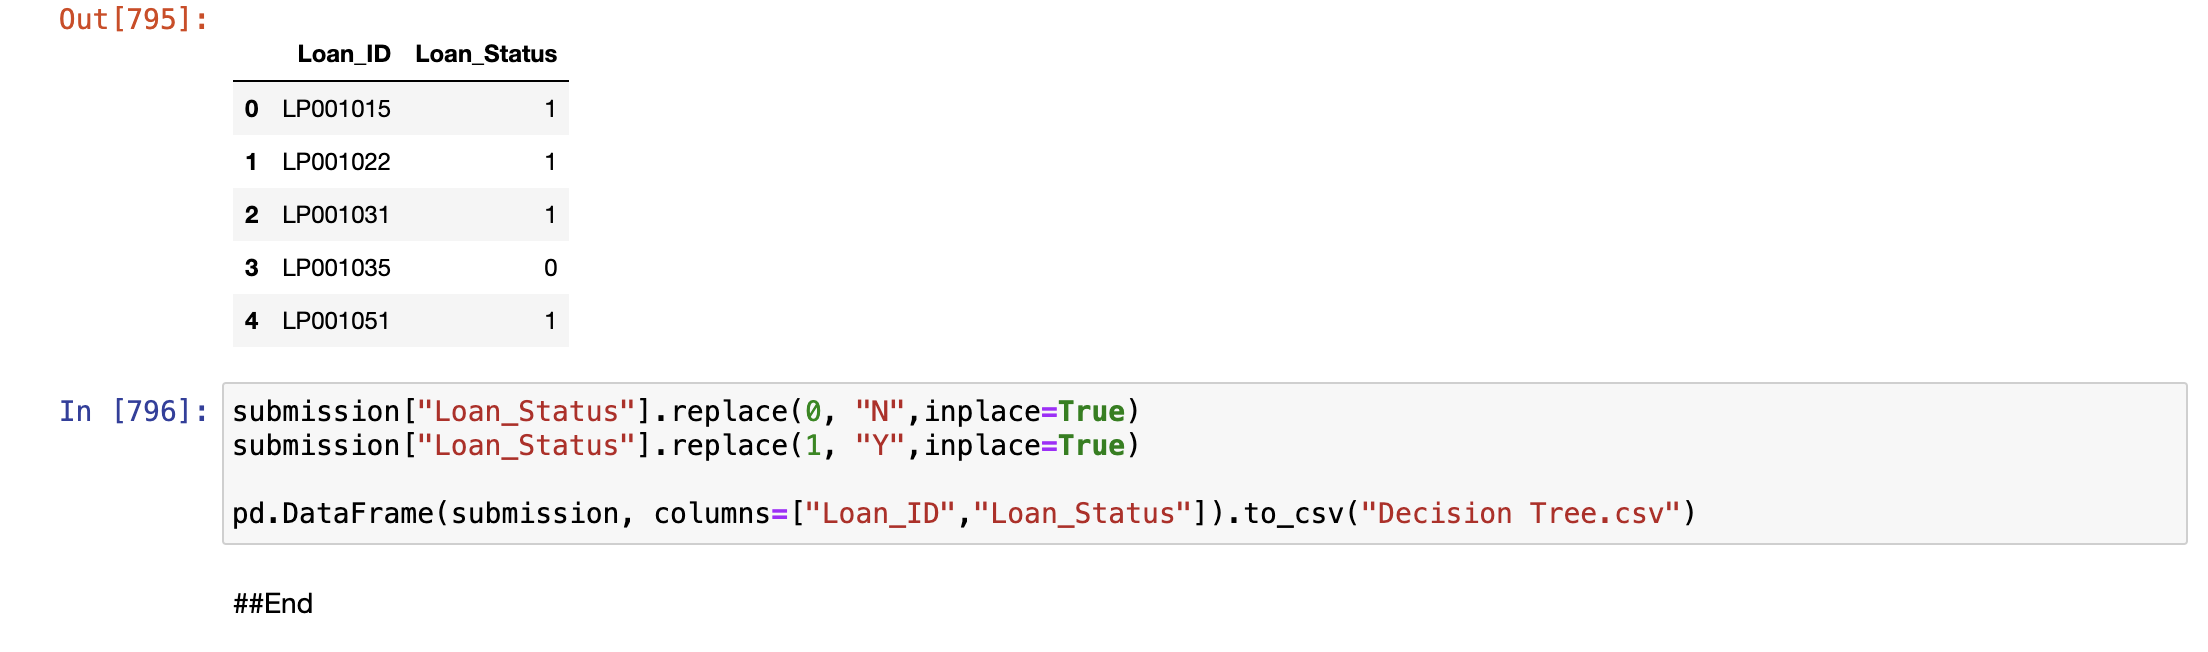
\includegraphics[width=\linewidth]{Decision_Tree_3.png}
        \label{fig:sub1}
\end{center}
\end{figure}
\end{enumerate}


\section*{Evaluation}

The performance of the loan prediction system is rigorously evaluated using accuracy metrics to ensure the reliability and effectiveness of the implemented machine learning models.

\subsection*{Evaluation Metrics}

The following key evaluation metric is employed to assess the performance of the models:

\begin{itemize}
    \item \textbf{Accuracy:} The ratio of correctly predicted instances to the total instances.
\end{itemize}

\subsection*{Results}

The performance of the machine learning models — Logistic Regression, Decision Trees, and K-Means Clustering — is evaluated on the test dataset using the aforementioned metrics. The results are summarized below:

\begin{table}[h]
    \centering
    \begin{tabular}{|l|c|c|c|c|}
        \hline
        \textbf{Model} & \textbf{Accuracy}\\
        \hline
        Logistic Regression & 0.83 \\
        Decision Trees & 0.64 \\
        K-Means Clustering & 0.80 \\
        \hline
    \end{tabular}
    \caption{Performance Metrics for Machine Learning Models}
    \label{tab:performance}
\end{table}

The results indicate that the Logistic Regression model outperforms the other models in terms of accuracy.  K-Means Clustering, originally designed for clustering tasks also exhibit reasonable performance, Decision Tree may not be the optimal choice for the problem at hand.


\subsection*{Conclusion}
In conclusion, the Loan Prediction Analysis for Banks project represents a significant stride towards addressing the critical challenges faced by lending institutions in the ever-evolving financial landscape. By harnessing the power of machine learning, we have successfully developed predictive models that contribute to more informed decision-making in the loan approval process.

The project aimed to answer the fundamental questions plaguing the lending industry:\\ 
How risky is the borrower, and should a loan be granted based on this risk assessment?\\
Through extensive exploration of various machine learning algorithms and methodologies, we have crafted a robust predictive system that leverages historical data to accurately evaluate the creditworthiness of loan applicants.

The implementation of the Loan Prediction System not only enhances the accuracy of risk assessment but also streamlines operational processes within banks. By significantly reducing the reliance on manual efforts and optimizing resource utilization, the system serves as a beacon of efficiency in an industry where time and precision are of the essence.

Real-world testing and evaluation have demonstrated the effectiveness of our predictive models, providing a tangible solution to the challenges faced by banks in the loan approval domain. The measured metrics, including accuracy attest to the reliability of the system in making informed predictions.

As we embrace the outcomes of this project, it is essential to acknowledge that the landscape of data and technology is dynamic.

In essence, the Loan Prediction Analysis for Banks project not only marks a successful integration of machine learning into financial decision-making but also serves as a foundation for ongoing advancements in predictive analytics within the banking industry. As we look ahead, the commitment to innovation and adaptability will be crucial in ensuring the sustained effectiveness and relevance of the Loan Prediction System in the face of changing economic landscapes and banking paradigms.
\end{document}